\documentclass[11pt]{article}

    \usepackage[breakable]{tcolorbox}
    \usepackage{parskip} % Stop auto-indenting (to mimic markdown behaviour)
    
    \usepackage{iftex}
    \ifPDFTeX
    	\usepackage[T1]{fontenc}
    	\usepackage{mathpazo}
    \else
    	\usepackage{fontspec}
    \fi

    % Basic figure setup, for now with no caption control since it's done
    % automatically by Pandoc (which extracts ![](path) syntax from Markdown).
    \usepackage{graphicx}
    % Maintain compatibility with old templates. Remove in nbconvert 6.0
    \let\Oldincludegraphics\includegraphics
    % Ensure that by default, figures have no caption (until we provide a
    % proper Figure object with a Caption API and a way to capture that
    % in the conversion process - todo).
    \usepackage{caption}
    \DeclareCaptionFormat{nocaption}{}
    \captionsetup{format=nocaption,aboveskip=0pt,belowskip=0pt}

    \usepackage{float}
    \floatplacement{figure}{H} % forces figures to be placed at the correct location
    \usepackage{xcolor} % Allow colors to be defined
    \usepackage{enumerate} % Needed for markdown enumerations to work
    \usepackage{geometry} % Used to adjust the document margins
    \usepackage{amsmath} % Equations
    \usepackage{amssymb} % Equations
    \usepackage{textcomp} % defines textquotesingle
    % Hack from http://tex.stackexchange.com/a/47451/13684:
    \AtBeginDocument{%
        \def\PYZsq{\textquotesingle}% Upright quotes in Pygmentized code
    }
    \usepackage{upquote} % Upright quotes for verbatim code
    \usepackage{eurosym} % defines \euro
    \usepackage[mathletters]{ucs} % Extended unicode (utf-8) support
    \usepackage{fancyvrb} % verbatim replacement that allows latex
    \usepackage{grffile} % extends the file name processing of package graphics 
                         % to support a larger range
    \makeatletter % fix for old versions of grffile with XeLaTeX
    \@ifpackagelater{grffile}{2019/11/01}
    {
      % Do nothing on new versions
    }
    {
      \def\Gread@@xetex#1{%
        \IfFileExists{"\Gin@base".bb}%
        {\Gread@eps{\Gin@base.bb}}%
        {\Gread@@xetex@aux#1}%
      }
    }
    \makeatother
    \usepackage[Export]{adjustbox} % Used to constrain images to a maximum size
    \adjustboxset{max size={0.9\linewidth}{0.9\paperheight}}

    % The hyperref package gives us a pdf with properly built
    % internal navigation ('pdf bookmarks' for the table of contents,
    % internal cross-reference links, web links for URLs, etc.)
    \usepackage{hyperref}
    % The default LaTeX title has an obnoxious amount of whitespace. By default,
    % titling removes some of it. It also provides customization options.
    \usepackage{titling}
    \usepackage{longtable} % longtable support required by pandoc >1.10
    \usepackage{booktabs}  % table support for pandoc > 1.12.2
    \usepackage[inline]{enumitem} % IRkernel/repr support (it uses the enumerate* environment)
    \usepackage[normalem]{ulem} % ulem is needed to support strikethroughs (\sout)
                                % normalem makes italics be italics, not underlines
    \usepackage{mathrsfs}
    

    
    % Colors for the hyperref package
    \definecolor{urlcolor}{rgb}{0,.145,.698}
    \definecolor{linkcolor}{rgb}{.71,0.21,0.01}
    \definecolor{citecolor}{rgb}{.12,.54,.11}

    % ANSI colors
    \definecolor{ansi-black}{HTML}{3E424D}
    \definecolor{ansi-black-intense}{HTML}{282C36}
    \definecolor{ansi-red}{HTML}{E75C58}
    \definecolor{ansi-red-intense}{HTML}{B22B31}
    \definecolor{ansi-green}{HTML}{00A250}
    \definecolor{ansi-green-intense}{HTML}{007427}
    \definecolor{ansi-yellow}{HTML}{DDB62B}
    \definecolor{ansi-yellow-intense}{HTML}{B27D12}
    \definecolor{ansi-blue}{HTML}{208FFB}
    \definecolor{ansi-blue-intense}{HTML}{0065CA}
    \definecolor{ansi-magenta}{HTML}{D160C4}
    \definecolor{ansi-magenta-intense}{HTML}{A03196}
    \definecolor{ansi-cyan}{HTML}{60C6C8}
    \definecolor{ansi-cyan-intense}{HTML}{258F8F}
    \definecolor{ansi-white}{HTML}{C5C1B4}
    \definecolor{ansi-white-intense}{HTML}{A1A6B2}
    \definecolor{ansi-default-inverse-fg}{HTML}{FFFFFF}
    \definecolor{ansi-default-inverse-bg}{HTML}{000000}

    % common color for the border for error outputs.
    \definecolor{outerrorbackground}{HTML}{FFDFDF}

    % commands and environments needed by pandoc snippets
    % extracted from the output of `pandoc -s`
    \providecommand{\tightlist}{%
      \setlength{\itemsep}{0pt}\setlength{\parskip}{0pt}}
    \DefineVerbatimEnvironment{Highlighting}{Verbatim}{commandchars=\\\{\}}
    % Add ',fontsize=\small' for more characters per line
    \newenvironment{Shaded}{}{}
    \newcommand{\KeywordTok}[1]{\textcolor[rgb]{0.00,0.44,0.13}{\textbf{{#1}}}}
    \newcommand{\DataTypeTok}[1]{\textcolor[rgb]{0.56,0.13,0.00}{{#1}}}
    \newcommand{\DecValTok}[1]{\textcolor[rgb]{0.25,0.63,0.44}{{#1}}}
    \newcommand{\BaseNTok}[1]{\textcolor[rgb]{0.25,0.63,0.44}{{#1}}}
    \newcommand{\FloatTok}[1]{\textcolor[rgb]{0.25,0.63,0.44}{{#1}}}
    \newcommand{\CharTok}[1]{\textcolor[rgb]{0.25,0.44,0.63}{{#1}}}
    \newcommand{\StringTok}[1]{\textcolor[rgb]{0.25,0.44,0.63}{{#1}}}
    \newcommand{\CommentTok}[1]{\textcolor[rgb]{0.38,0.63,0.69}{\textit{{#1}}}}
    \newcommand{\OtherTok}[1]{\textcolor[rgb]{0.00,0.44,0.13}{{#1}}}
    \newcommand{\AlertTok}[1]{\textcolor[rgb]{1.00,0.00,0.00}{\textbf{{#1}}}}
    \newcommand{\FunctionTok}[1]{\textcolor[rgb]{0.02,0.16,0.49}{{#1}}}
    \newcommand{\RegionMarkerTok}[1]{{#1}}
    \newcommand{\ErrorTok}[1]{\textcolor[rgb]{1.00,0.00,0.00}{\textbf{{#1}}}}
    \newcommand{\NormalTok}[1]{{#1}}
    
    % Additional commands for more recent versions of Pandoc
    \newcommand{\ConstantTok}[1]{\textcolor[rgb]{0.53,0.00,0.00}{{#1}}}
    \newcommand{\SpecialCharTok}[1]{\textcolor[rgb]{0.25,0.44,0.63}{{#1}}}
    \newcommand{\VerbatimStringTok}[1]{\textcolor[rgb]{0.25,0.44,0.63}{{#1}}}
    \newcommand{\SpecialStringTok}[1]{\textcolor[rgb]{0.73,0.40,0.53}{{#1}}}
    \newcommand{\ImportTok}[1]{{#1}}
    \newcommand{\DocumentationTok}[1]{\textcolor[rgb]{0.73,0.13,0.13}{\textit{{#1}}}}
    \newcommand{\AnnotationTok}[1]{\textcolor[rgb]{0.38,0.63,0.69}{\textbf{\textit{{#1}}}}}
    \newcommand{\CommentVarTok}[1]{\textcolor[rgb]{0.38,0.63,0.69}{\textbf{\textit{{#1}}}}}
    \newcommand{\VariableTok}[1]{\textcolor[rgb]{0.10,0.09,0.49}{{#1}}}
    \newcommand{\ControlFlowTok}[1]{\textcolor[rgb]{0.00,0.44,0.13}{\textbf{{#1}}}}
    \newcommand{\OperatorTok}[1]{\textcolor[rgb]{0.40,0.40,0.40}{{#1}}}
    \newcommand{\BuiltInTok}[1]{{#1}}
    \newcommand{\ExtensionTok}[1]{{#1}}
    \newcommand{\PreprocessorTok}[1]{\textcolor[rgb]{0.74,0.48,0.00}{{#1}}}
    \newcommand{\AttributeTok}[1]{\textcolor[rgb]{0.49,0.56,0.16}{{#1}}}
    \newcommand{\InformationTok}[1]{\textcolor[rgb]{0.38,0.63,0.69}{\textbf{\textit{{#1}}}}}
    \newcommand{\WarningTok}[1]{\textcolor[rgb]{0.38,0.63,0.69}{\textbf{\textit{{#1}}}}}
    
    
    % Define a nice break command that doesn't care if a line doesn't already
    % exist.
    \def\br{\hspace*{\fill} \\* }
    % Math Jax compatibility definitions
    \def\gt{>}
    \def\lt{<}
    \let\Oldtex\TeX
    \let\Oldlatex\LaTeX
    \renewcommand{\TeX}{\textrm{\Oldtex}}
    \renewcommand{\LaTeX}{\textrm{\Oldlatex}}
    % Document parameters
    % Document title
    \title{SWNM}
    
    
    
    
    
% Pygments definitions
\makeatletter
\def\PY@reset{\let\PY@it=\relax \let\PY@bf=\relax%
    \let\PY@ul=\relax \let\PY@tc=\relax%
    \let\PY@bc=\relax \let\PY@ff=\relax}
\def\PY@tok#1{\csname PY@tok@#1\endcsname}
\def\PY@toks#1+{\ifx\relax#1\empty\else%
    \PY@tok{#1}\expandafter\PY@toks\fi}
\def\PY@do#1{\PY@bc{\PY@tc{\PY@ul{%
    \PY@it{\PY@bf{\PY@ff{#1}}}}}}}
\def\PY#1#2{\PY@reset\PY@toks#1+\relax+\PY@do{#2}}

\expandafter\def\csname PY@tok@w\endcsname{\def\PY@tc##1{\textcolor[rgb]{0.73,0.73,0.73}{##1}}}
\expandafter\def\csname PY@tok@c\endcsname{\let\PY@it=\textit\def\PY@tc##1{\textcolor[rgb]{0.25,0.50,0.50}{##1}}}
\expandafter\def\csname PY@tok@cp\endcsname{\def\PY@tc##1{\textcolor[rgb]{0.74,0.48,0.00}{##1}}}
\expandafter\def\csname PY@tok@k\endcsname{\let\PY@bf=\textbf\def\PY@tc##1{\textcolor[rgb]{0.00,0.50,0.00}{##1}}}
\expandafter\def\csname PY@tok@kp\endcsname{\def\PY@tc##1{\textcolor[rgb]{0.00,0.50,0.00}{##1}}}
\expandafter\def\csname PY@tok@kt\endcsname{\def\PY@tc##1{\textcolor[rgb]{0.69,0.00,0.25}{##1}}}
\expandafter\def\csname PY@tok@o\endcsname{\def\PY@tc##1{\textcolor[rgb]{0.40,0.40,0.40}{##1}}}
\expandafter\def\csname PY@tok@ow\endcsname{\let\PY@bf=\textbf\def\PY@tc##1{\textcolor[rgb]{0.67,0.13,1.00}{##1}}}
\expandafter\def\csname PY@tok@nb\endcsname{\def\PY@tc##1{\textcolor[rgb]{0.00,0.50,0.00}{##1}}}
\expandafter\def\csname PY@tok@nf\endcsname{\def\PY@tc##1{\textcolor[rgb]{0.00,0.00,1.00}{##1}}}
\expandafter\def\csname PY@tok@nc\endcsname{\let\PY@bf=\textbf\def\PY@tc##1{\textcolor[rgb]{0.00,0.00,1.00}{##1}}}
\expandafter\def\csname PY@tok@nn\endcsname{\let\PY@bf=\textbf\def\PY@tc##1{\textcolor[rgb]{0.00,0.00,1.00}{##1}}}
\expandafter\def\csname PY@tok@ne\endcsname{\let\PY@bf=\textbf\def\PY@tc##1{\textcolor[rgb]{0.82,0.25,0.23}{##1}}}
\expandafter\def\csname PY@tok@nv\endcsname{\def\PY@tc##1{\textcolor[rgb]{0.10,0.09,0.49}{##1}}}
\expandafter\def\csname PY@tok@no\endcsname{\def\PY@tc##1{\textcolor[rgb]{0.53,0.00,0.00}{##1}}}
\expandafter\def\csname PY@tok@nl\endcsname{\def\PY@tc##1{\textcolor[rgb]{0.63,0.63,0.00}{##1}}}
\expandafter\def\csname PY@tok@ni\endcsname{\let\PY@bf=\textbf\def\PY@tc##1{\textcolor[rgb]{0.60,0.60,0.60}{##1}}}
\expandafter\def\csname PY@tok@na\endcsname{\def\PY@tc##1{\textcolor[rgb]{0.49,0.56,0.16}{##1}}}
\expandafter\def\csname PY@tok@nt\endcsname{\let\PY@bf=\textbf\def\PY@tc##1{\textcolor[rgb]{0.00,0.50,0.00}{##1}}}
\expandafter\def\csname PY@tok@nd\endcsname{\def\PY@tc##1{\textcolor[rgb]{0.67,0.13,1.00}{##1}}}
\expandafter\def\csname PY@tok@s\endcsname{\def\PY@tc##1{\textcolor[rgb]{0.73,0.13,0.13}{##1}}}
\expandafter\def\csname PY@tok@sd\endcsname{\let\PY@it=\textit\def\PY@tc##1{\textcolor[rgb]{0.73,0.13,0.13}{##1}}}
\expandafter\def\csname PY@tok@si\endcsname{\let\PY@bf=\textbf\def\PY@tc##1{\textcolor[rgb]{0.73,0.40,0.53}{##1}}}
\expandafter\def\csname PY@tok@se\endcsname{\let\PY@bf=\textbf\def\PY@tc##1{\textcolor[rgb]{0.73,0.40,0.13}{##1}}}
\expandafter\def\csname PY@tok@sr\endcsname{\def\PY@tc##1{\textcolor[rgb]{0.73,0.40,0.53}{##1}}}
\expandafter\def\csname PY@tok@ss\endcsname{\def\PY@tc##1{\textcolor[rgb]{0.10,0.09,0.49}{##1}}}
\expandafter\def\csname PY@tok@sx\endcsname{\def\PY@tc##1{\textcolor[rgb]{0.00,0.50,0.00}{##1}}}
\expandafter\def\csname PY@tok@m\endcsname{\def\PY@tc##1{\textcolor[rgb]{0.40,0.40,0.40}{##1}}}
\expandafter\def\csname PY@tok@gh\endcsname{\let\PY@bf=\textbf\def\PY@tc##1{\textcolor[rgb]{0.00,0.00,0.50}{##1}}}
\expandafter\def\csname PY@tok@gu\endcsname{\let\PY@bf=\textbf\def\PY@tc##1{\textcolor[rgb]{0.50,0.00,0.50}{##1}}}
\expandafter\def\csname PY@tok@gd\endcsname{\def\PY@tc##1{\textcolor[rgb]{0.63,0.00,0.00}{##1}}}
\expandafter\def\csname PY@tok@gi\endcsname{\def\PY@tc##1{\textcolor[rgb]{0.00,0.63,0.00}{##1}}}
\expandafter\def\csname PY@tok@gr\endcsname{\def\PY@tc##1{\textcolor[rgb]{1.00,0.00,0.00}{##1}}}
\expandafter\def\csname PY@tok@ge\endcsname{\let\PY@it=\textit}
\expandafter\def\csname PY@tok@gs\endcsname{\let\PY@bf=\textbf}
\expandafter\def\csname PY@tok@gp\endcsname{\let\PY@bf=\textbf\def\PY@tc##1{\textcolor[rgb]{0.00,0.00,0.50}{##1}}}
\expandafter\def\csname PY@tok@go\endcsname{\def\PY@tc##1{\textcolor[rgb]{0.53,0.53,0.53}{##1}}}
\expandafter\def\csname PY@tok@gt\endcsname{\def\PY@tc##1{\textcolor[rgb]{0.00,0.27,0.87}{##1}}}
\expandafter\def\csname PY@tok@err\endcsname{\def\PY@bc##1{\setlength{\fboxsep}{0pt}\fcolorbox[rgb]{1.00,0.00,0.00}{1,1,1}{\strut ##1}}}
\expandafter\def\csname PY@tok@kc\endcsname{\let\PY@bf=\textbf\def\PY@tc##1{\textcolor[rgb]{0.00,0.50,0.00}{##1}}}
\expandafter\def\csname PY@tok@kd\endcsname{\let\PY@bf=\textbf\def\PY@tc##1{\textcolor[rgb]{0.00,0.50,0.00}{##1}}}
\expandafter\def\csname PY@tok@kn\endcsname{\let\PY@bf=\textbf\def\PY@tc##1{\textcolor[rgb]{0.00,0.50,0.00}{##1}}}
\expandafter\def\csname PY@tok@kr\endcsname{\let\PY@bf=\textbf\def\PY@tc##1{\textcolor[rgb]{0.00,0.50,0.00}{##1}}}
\expandafter\def\csname PY@tok@bp\endcsname{\def\PY@tc##1{\textcolor[rgb]{0.00,0.50,0.00}{##1}}}
\expandafter\def\csname PY@tok@fm\endcsname{\def\PY@tc##1{\textcolor[rgb]{0.00,0.00,1.00}{##1}}}
\expandafter\def\csname PY@tok@vc\endcsname{\def\PY@tc##1{\textcolor[rgb]{0.10,0.09,0.49}{##1}}}
\expandafter\def\csname PY@tok@vg\endcsname{\def\PY@tc##1{\textcolor[rgb]{0.10,0.09,0.49}{##1}}}
\expandafter\def\csname PY@tok@vi\endcsname{\def\PY@tc##1{\textcolor[rgb]{0.10,0.09,0.49}{##1}}}
\expandafter\def\csname PY@tok@vm\endcsname{\def\PY@tc##1{\textcolor[rgb]{0.10,0.09,0.49}{##1}}}
\expandafter\def\csname PY@tok@sa\endcsname{\def\PY@tc##1{\textcolor[rgb]{0.73,0.13,0.13}{##1}}}
\expandafter\def\csname PY@tok@sb\endcsname{\def\PY@tc##1{\textcolor[rgb]{0.73,0.13,0.13}{##1}}}
\expandafter\def\csname PY@tok@sc\endcsname{\def\PY@tc##1{\textcolor[rgb]{0.73,0.13,0.13}{##1}}}
\expandafter\def\csname PY@tok@dl\endcsname{\def\PY@tc##1{\textcolor[rgb]{0.73,0.13,0.13}{##1}}}
\expandafter\def\csname PY@tok@s2\endcsname{\def\PY@tc##1{\textcolor[rgb]{0.73,0.13,0.13}{##1}}}
\expandafter\def\csname PY@tok@sh\endcsname{\def\PY@tc##1{\textcolor[rgb]{0.73,0.13,0.13}{##1}}}
\expandafter\def\csname PY@tok@s1\endcsname{\def\PY@tc##1{\textcolor[rgb]{0.73,0.13,0.13}{##1}}}
\expandafter\def\csname PY@tok@mb\endcsname{\def\PY@tc##1{\textcolor[rgb]{0.40,0.40,0.40}{##1}}}
\expandafter\def\csname PY@tok@mf\endcsname{\def\PY@tc##1{\textcolor[rgb]{0.40,0.40,0.40}{##1}}}
\expandafter\def\csname PY@tok@mh\endcsname{\def\PY@tc##1{\textcolor[rgb]{0.40,0.40,0.40}{##1}}}
\expandafter\def\csname PY@tok@mi\endcsname{\def\PY@tc##1{\textcolor[rgb]{0.40,0.40,0.40}{##1}}}
\expandafter\def\csname PY@tok@il\endcsname{\def\PY@tc##1{\textcolor[rgb]{0.40,0.40,0.40}{##1}}}
\expandafter\def\csname PY@tok@mo\endcsname{\def\PY@tc##1{\textcolor[rgb]{0.40,0.40,0.40}{##1}}}
\expandafter\def\csname PY@tok@ch\endcsname{\let\PY@it=\textit\def\PY@tc##1{\textcolor[rgb]{0.25,0.50,0.50}{##1}}}
\expandafter\def\csname PY@tok@cm\endcsname{\let\PY@it=\textit\def\PY@tc##1{\textcolor[rgb]{0.25,0.50,0.50}{##1}}}
\expandafter\def\csname PY@tok@cpf\endcsname{\let\PY@it=\textit\def\PY@tc##1{\textcolor[rgb]{0.25,0.50,0.50}{##1}}}
\expandafter\def\csname PY@tok@c1\endcsname{\let\PY@it=\textit\def\PY@tc##1{\textcolor[rgb]{0.25,0.50,0.50}{##1}}}
\expandafter\def\csname PY@tok@cs\endcsname{\let\PY@it=\textit\def\PY@tc##1{\textcolor[rgb]{0.25,0.50,0.50}{##1}}}

\def\PYZbs{\char`\\}
\def\PYZus{\char`\_}
\def\PYZob{\char`\{}
\def\PYZcb{\char`\}}
\def\PYZca{\char`\^}
\def\PYZam{\char`\&}
\def\PYZlt{\char`\<}
\def\PYZgt{\char`\>}
\def\PYZsh{\char`\#}
\def\PYZpc{\char`\%}
\def\PYZdl{\char`\$}
\def\PYZhy{\char`\-}
\def\PYZsq{\char`\'}
\def\PYZdq{\char`\"}
\def\PYZti{\char`\~}
% for compatibility with earlier versions
\def\PYZat{@}
\def\PYZlb{[}
\def\PYZrb{]}
\makeatother


    % For linebreaks inside Verbatim environment from package fancyvrb. 
    \makeatletter
        \newbox\Wrappedcontinuationbox 
        \newbox\Wrappedvisiblespacebox 
        \newcommand*\Wrappedvisiblespace {\textcolor{red}{\textvisiblespace}} 
        \newcommand*\Wrappedcontinuationsymbol {\textcolor{red}{\llap{\tiny$\m@th\hookrightarrow$}}} 
        \newcommand*\Wrappedcontinuationindent {3ex } 
        \newcommand*\Wrappedafterbreak {\kern\Wrappedcontinuationindent\copy\Wrappedcontinuationbox} 
        % Take advantage of the already applied Pygments mark-up to insert 
        % potential linebreaks for TeX processing. 
        %        {, <, #, %, $, ' and ": go to next line. 
        %        _, }, ^, &, >, - and ~: stay at end of broken line. 
        % Use of \textquotesingle for straight quote. 
        \newcommand*\Wrappedbreaksatspecials {% 
            \def\PYGZus{\discretionary{\char`\_}{\Wrappedafterbreak}{\char`\_}}% 
            \def\PYGZob{\discretionary{}{\Wrappedafterbreak\char`\{}{\char`\{}}% 
            \def\PYGZcb{\discretionary{\char`\}}{\Wrappedafterbreak}{\char`\}}}% 
            \def\PYGZca{\discretionary{\char`\^}{\Wrappedafterbreak}{\char`\^}}% 
            \def\PYGZam{\discretionary{\char`\&}{\Wrappedafterbreak}{\char`\&}}% 
            \def\PYGZlt{\discretionary{}{\Wrappedafterbreak\char`\<}{\char`\<}}% 
            \def\PYGZgt{\discretionary{\char`\>}{\Wrappedafterbreak}{\char`\>}}% 
            \def\PYGZsh{\discretionary{}{\Wrappedafterbreak\char`\#}{\char`\#}}% 
            \def\PYGZpc{\discretionary{}{\Wrappedafterbreak\char`\%}{\char`\%}}% 
            \def\PYGZdl{\discretionary{}{\Wrappedafterbreak\char`\$}{\char`\$}}% 
            \def\PYGZhy{\discretionary{\char`\-}{\Wrappedafterbreak}{\char`\-}}% 
            \def\PYGZsq{\discretionary{}{\Wrappedafterbreak\textquotesingle}{\textquotesingle}}% 
            \def\PYGZdq{\discretionary{}{\Wrappedafterbreak\char`\"}{\char`\"}}% 
            \def\PYGZti{\discretionary{\char`\~}{\Wrappedafterbreak}{\char`\~}}% 
        } 
        % Some characters . , ; ? ! / are not pygmentized. 
        % This macro makes them "active" and they will insert potential linebreaks 
        \newcommand*\Wrappedbreaksatpunct {% 
            \lccode`\~`\.\lowercase{\def~}{\discretionary{\hbox{\char`\.}}{\Wrappedafterbreak}{\hbox{\char`\.}}}% 
            \lccode`\~`\,\lowercase{\def~}{\discretionary{\hbox{\char`\,}}{\Wrappedafterbreak}{\hbox{\char`\,}}}% 
            \lccode`\~`\;\lowercase{\def~}{\discretionary{\hbox{\char`\;}}{\Wrappedafterbreak}{\hbox{\char`\;}}}% 
            \lccode`\~`\:\lowercase{\def~}{\discretionary{\hbox{\char`\:}}{\Wrappedafterbreak}{\hbox{\char`\:}}}% 
            \lccode`\~`\?\lowercase{\def~}{\discretionary{\hbox{\char`\?}}{\Wrappedafterbreak}{\hbox{\char`\?}}}% 
            \lccode`\~`\!\lowercase{\def~}{\discretionary{\hbox{\char`\!}}{\Wrappedafterbreak}{\hbox{\char`\!}}}% 
            \lccode`\~`\/\lowercase{\def~}{\discretionary{\hbox{\char`\/}}{\Wrappedafterbreak}{\hbox{\char`\/}}}% 
            \catcode`\.\active
            \catcode`\,\active 
            \catcode`\;\active
            \catcode`\:\active
            \catcode`\?\active
            \catcode`\!\active
            \catcode`\/\active 
            \lccode`\~`\~ 	
        }
    \makeatother

    \let\OriginalVerbatim=\Verbatim
    \makeatletter
    \renewcommand{\Verbatim}[1][1]{%
        %\parskip\z@skip
        \sbox\Wrappedcontinuationbox {\Wrappedcontinuationsymbol}%
        \sbox\Wrappedvisiblespacebox {\FV@SetupFont\Wrappedvisiblespace}%
        \def\FancyVerbFormatLine ##1{\hsize\linewidth
            \vtop{\raggedright\hyphenpenalty\z@\exhyphenpenalty\z@
                \doublehyphendemerits\z@\finalhyphendemerits\z@
                \strut ##1\strut}%
        }%
        % If the linebreak is at a space, the latter will be displayed as visible
        % space at end of first line, and a continuation symbol starts next line.
        % Stretch/shrink are however usually zero for typewriter font.
        \def\FV@Space {%
            \nobreak\hskip\z@ plus\fontdimen3\font minus\fontdimen4\font
            \discretionary{\copy\Wrappedvisiblespacebox}{\Wrappedafterbreak}
            {\kern\fontdimen2\font}%
        }%
        
        % Allow breaks at special characters using \PYG... macros.
        \Wrappedbreaksatspecials
        % Breaks at punctuation characters . , ; ? ! and / need catcode=\active 	
        \OriginalVerbatim[#1,codes*=\Wrappedbreaksatpunct]%
    }
    \makeatother

    % Exact colors from NB
    \definecolor{incolor}{HTML}{303F9F}
    \definecolor{outcolor}{HTML}{D84315}
    \definecolor{cellborder}{HTML}{CFCFCF}
    \definecolor{cellbackground}{HTML}{F7F7F7}
    
    % prompt
    \makeatletter
    \newcommand{\boxspacing}{\kern\kvtcb@left@rule\kern\kvtcb@boxsep}
    \makeatother
    \newcommand{\prompt}[4]{
        {\ttfamily\llap{{\color{#2}[#3]:\hspace{3pt}#4}}\vspace{-\baselineskip}}
    }
    

    
    % Prevent overflowing lines due to hard-to-break entities
    \sloppy 
    % Setup hyperref package
    \hypersetup{
      breaklinks=true,  % so long urls are correctly broken across lines
      colorlinks=true,
      urlcolor=urlcolor,
      linkcolor=linkcolor,
      citecolor=citecolor,
      }
    % Slightly bigger margins than the latex defaults
    
    \geometry{verbose,tmargin=1in,bmargin=1in,lmargin=1in,rmargin=1in}
    
    

\begin{document}
    
    \maketitle
    
    

    
    \hypertarget{geothermal-machine-learning-analysis-southwest-new-mexico}{%
\subsection{Geothermal machine learning analysis: Southwest New
Mexico}\label{geothermal-machine-learning-analysis-southwest-new-mexico}}

This notebook is a part of the GTcloud.jl: GeoThermal Cloud for Machine
Learning.

\begin{verbatim}
<img src="../../logos/geothermalcloud-small.png" alt="geothermalcloud" width=25%  max-width=125px;/>
\end{verbatim}

Machine learning analyses are performed using the \textbf{SmartTensors}
machine learning framework.

\begin{verbatim}
<img src="../../logos/SmartTensorsNewSmaller.png" alt="SmartTensors" width=25%  max-width=125px;/>
\end{verbatim}

This notebook demonstrates how the \textbf{NMFk} module of
\textbf{SmartTensors} can be applied to perform unsupervised geothermal
machine-learning analyses.

\begin{verbatim}
<img src="../../logos/nmfk-logo.png" alt="nmfk" width=25%  max-width=125px;/>
\end{verbatim}

More information how the ML results are interpreted to provide
geothermal insights is discussed in our research paper.

    \hypertarget{import-required-libraries-for-this-work}{%
\subsection{Import required libraries for this
work}\label{import-required-libraries-for-this-work}}

If \textbf{NMFk} is not installed, first execute in the Julia REPL
\texttt{import\ Pkg;\ Pkg.add("NMFk");\ Pkg.add("DelimitedFiles");\ Pkg.add("JLD");\ Pkg.add("Gadfly");\ Pkg.add("Cairo");\ Pkg.add("Fontconfig");\ Pkg.add("Mads")}.

    \begin{tcolorbox}[breakable, size=fbox, boxrule=1pt, pad at break*=1mm,colback=cellbackground, colframe=cellborder]
\prompt{In}{incolor}{1}{\boxspacing}
\begin{Verbatim}[commandchars=\\\{\}]
\PY{k+kn}{import} \PY{n+nn}{NMFk}
\PY{k+kn}{import} \PY{n+nn}{DelimitedFiles}
\PY{k+kn}{import} \PY{n+nn}{JLD}
\PY{k+kn}{import} \PY{n+nn}{Gadfly}
\PY{k+kn}{import} \PY{n+nn}{Cairo}
\PY{k+kn}{import} \PY{n+nn}{Fontconfig}
\PY{k+kn}{import} \PY{n+nn}{Mads}
\end{Verbatim}
\end{tcolorbox}

    \hypertarget{load-and-pre-process-the-data}{%
\subsection{Load and pre-process the
data}\label{load-and-pre-process-the-data}}

    \hypertarget{setup-the-working-directory-containing-the-swnm-data}{%
\subsubsection{Setup the working directory containing the SWNM
data}\label{setup-the-working-directory-containing-the-swnm-data}}

    \begin{tcolorbox}[breakable, size=fbox, boxrule=1pt, pad at break*=1mm,colback=cellbackground, colframe=cellborder]
\prompt{In}{incolor}{2}{\boxspacing}
\begin{Verbatim}[commandchars=\\\{\}]
\PY{n}{cd}\PY{p}{(}\PY{l+s+s2}{\PYZdq{}}\PY{l+s+s2}{/Users/vvv/Julia/GTcloud\PYZhy{}SmartTensors.jl/SWNM}\PY{l+s+s2}{\PYZdq{}}\PY{p}{)}\PY{p}{;}
\end{Verbatim}
\end{tcolorbox}

    \hypertarget{load-the-data-file}{%
\subsubsection{Load the data file}\label{load-the-data-file}}

    \begin{tcolorbox}[breakable, size=fbox, boxrule=1pt, pad at break*=1mm,colback=cellbackground, colframe=cellborder]
\prompt{In}{incolor}{3}{\boxspacing}
\begin{Verbatim}[commandchars=\\\{\}]
\PY{n}{d}\PY{p}{,} \PY{n}{h} \PY{o}{=} \PY{n}{DelimitedFiles}\PY{o}{.}\PY{n}{readdlm}\PY{p}{(}\PY{l+s+s2}{\PYZdq{}}\PY{l+s+s2}{data/Pepin\PYZus{}PCA\PYZus{}Input\PYZus{}Data\PYZus{}LANL.csv}\PY{l+s+s2}{\PYZdq{}}\PY{p}{,} \PY{l+s+s1}{\PYZsq{}}\PY{l+s+s1}{,}\PY{l+s+s1}{\PYZsq{}}\PY{p}{;} \PY{n}{header}\PY{o}{=}\PY{n}{true}\PY{p}{)}\PY{p}{;}
\end{Verbatim}
\end{tcolorbox}

    \hypertarget{define-names-of-the-data-attributes-matrix-columns}{%
\subsubsection{Define names of the data attributes (matrix
columns)}\label{define-names-of-the-data-attributes-matrix-columns}}

    \begin{tcolorbox}[breakable, size=fbox, boxrule=1pt, pad at break*=1mm,colback=cellbackground, colframe=cellborder]
\prompt{In}{incolor}{4}{\boxspacing}
\begin{Verbatim}[commandchars=\\\{\}]
\PY{n}{attributes\PYZus{}short} \PY{o}{=} \PY{p}{[}\PY{l+s+s2}{\PYZdq{}}\PY{l+s+s2}{Boron}\PY{l+s+s2}{\PYZdq{}}\PY{p}{;} \PY{l+s+s2}{\PYZdq{}}\PY{l+s+s2}{Gravity}\PY{l+s+s2}{\PYZdq{}}\PY{p}{;} \PY{l+s+s2}{\PYZdq{}}\PY{l+s+s2}{Magnetic}\PY{l+s+s2}{\PYZdq{}}\PY{p}{;} \PY{l+s+s2}{\PYZdq{}}\PY{l+s+s2}{Dikes}\PY{l+s+s2}{\PYZdq{}}\PY{p}{;} \PY{l+s+s2}{\PYZdq{}}\PY{l+s+s2}{Drainage}\PY{l+s+s2}{\PYZdq{}}\PY{p}{;} \PY{l+s+s2}{\PYZdq{}}\PY{l+s+s2}{FaultInter}\PY{l+s+s2}{\PYZdq{}}\PY{p}{;} \PY{l+s+s2}{\PYZdq{}}\PY{l+s+s2}{QuatFaults}\PY{l+s+s2}{\PYZdq{}}\PY{p}{;} \PY{l+s+s2}{\PYZdq{}}\PY{l+s+s2}{Seismicity}\PY{l+s+s2}{\PYZdq{}}\PY{p}{;} \PY{l+s+s2}{\PYZdq{}}\PY{l+s+s2}{NMFaults}\PY{l+s+s2}{\PYZdq{}}\PY{p}{;} \PY{l+s+s2}{\PYZdq{}}\PY{l+s+s2}{Springs}\PY{l+s+s2}{\PYZdq{}}\PY{p}{;} \PY{l+s+s2}{\PYZdq{}}\PY{l+s+s2}{Vents}\PY{l+s+s2}{\PYZdq{}}\PY{p}{;} \PY{l+s+s2}{\PYZdq{}}\PY{l+s+s2}{Lithium}\PY{l+s+s2}{\PYZdq{}}\PY{p}{;} \PY{l+s+s2}{\PYZdq{}}\PY{l+s+s2}{Precip}\PY{l+s+s2}{\PYZdq{}}\PY{p}{;} \PY{l+s+s2}{\PYZdq{}}\PY{l+s+s2}{Air\PYZus{}Temp}\PY{l+s+s2}{\PYZdq{}}\PY{p}{;} \PY{l+s+s2}{\PYZdq{}}\PY{l+s+s2}{Silica}\PY{l+s+s2}{\PYZdq{}}\PY{p}{;} \PY{l+s+s2}{\PYZdq{}}\PY{l+s+s2}{Subcrop}\PY{l+s+s2}{\PYZdq{}}\PY{p}{;} \PY{l+s+s2}{\PYZdq{}}\PY{l+s+s2}{WT\PYZus{}Gradient}\PY{l+s+s2}{\PYZdq{}}\PY{p}{;} \PY{l+s+s2}{\PYZdq{}}\PY{l+s+s2}{WT\PYZus{}Elev}\PY{l+s+s2}{\PYZdq{}}\PY{p}{;} \PY{l+s+s2}{\PYZdq{}}\PY{l+s+s2}{Heatflow}\PY{l+s+s2}{\PYZdq{}}\PY{p}{;} \PY{l+s+s2}{\PYZdq{}}\PY{l+s+s2}{GS\PYZus{}Elev}\PY{l+s+s2}{\PYZdq{}}\PY{p}{;} \PY{l+s+s2}{\PYZdq{}}\PY{l+s+s2}{DTW}\PY{l+s+s2}{\PYZdq{}}\PY{p}{;} \PY{l+s+s2}{\PYZdq{}}\PY{l+s+s2}{Crst\PYZus{}Thick}\PY{l+s+s2}{\PYZdq{}}\PY{p}{;} \PY{l+s+s2}{\PYZdq{}}\PY{l+s+s2}{Bsmt\PYZus{}Depth}\PY{l+s+s2}{\PYZdq{}}\PY{p}{]}
\PY{n}{attributes\PYZus{}long} \PY{o}{=} \PY{n}{uppercasefirst}\PY{o}{.}\PY{p}{(}\PY{n}{lowercase}\PY{o}{.}\PY{p}{(}\PY{p}{[}\PY{l+s+s2}{\PYZdq{}}\PY{l+s+s2}{Boron Concentration}\PY{l+s+s2}{\PYZdq{}}\PY{p}{;} \PY{l+s+s2}{\PYZdq{}}\PY{l+s+s2}{Gravity Anomaly}\PY{l+s+s2}{\PYZdq{}}\PY{p}{;} \PY{l+s+s2}{\PYZdq{}}\PY{l+s+s2}{Magnetic Intensity}\PY{l+s+s2}{\PYZdq{}}\PY{p}{;} \PY{l+s+s2}{\PYZdq{}}\PY{l+s+s2}{Volcanic Dike Density}\PY{l+s+s2}{\PYZdq{}}\PY{p}{;} \PY{l+s+s2}{\PYZdq{}}\PY{l+s+s2}{Drainage Density}\PY{l+s+s2}{\PYZdq{}}\PY{p}{;} \PY{l+s+s2}{\PYZdq{}}\PY{l+s+s2}{Fault Intersection Density}\PY{l+s+s2}{\PYZdq{}}\PY{p}{;} \PY{l+s+s2}{\PYZdq{}}\PY{l+s+s2}{Quaternary Fault Density}\PY{l+s+s2}{\PYZdq{}}\PY{p}{;} \PY{l+s+s2}{\PYZdq{}}\PY{l+s+s2}{Seismicity}\PY{l+s+s2}{\PYZdq{}}\PY{p}{;} \PY{l+s+s2}{\PYZdq{}}\PY{l+s+s2}{State Map Fault Density}\PY{l+s+s2}{\PYZdq{}}\PY{p}{;} \PY{l+s+s2}{\PYZdq{}}\PY{l+s+s2}{Spring Density}\PY{l+s+s2}{\PYZdq{}}\PY{p}{;} \PY{l+s+s2}{\PYZdq{}}\PY{l+s+s2}{Volcanic Vent Density}\PY{l+s+s2}{\PYZdq{}}\PY{p}{;} \PY{l+s+s2}{\PYZdq{}}\PY{l+s+s2}{Lithium Concentration}\PY{l+s+s2}{\PYZdq{}}\PY{p}{;} \PY{l+s+s2}{\PYZdq{}}\PY{l+s+s2}{Precipitation}\PY{l+s+s2}{\PYZdq{}}\PY{p}{;} \PY{l+s+s2}{\PYZdq{}}\PY{l+s+s2}{Air Temperature}\PY{l+s+s2}{\PYZdq{}}\PY{p}{;} \PY{l+s+s2}{\PYZdq{}}\PY{l+s+s2}{Silica Geothermometer}\PY{l+s+s2}{\PYZdq{}}\PY{p}{;} \PY{l+s+s2}{\PYZdq{}}\PY{l+s+s2}{Subcrop Permeability}\PY{l+s+s2}{\PYZdq{}}\PY{p}{;} \PY{l+s+s2}{\PYZdq{}}\PY{l+s+s2}{Hydraulic Gradient}\PY{l+s+s2}{\PYZdq{}}\PY{p}{;} \PY{l+s+s2}{\PYZdq{}}\PY{l+s+s2}{Watertable Elevation}\PY{l+s+s2}{\PYZdq{}}\PY{p}{;} \PY{l+s+s2}{\PYZdq{}}\PY{l+s+s2}{Heat flow}\PY{l+s+s2}{\PYZdq{}}\PY{p}{;} \PY{l+s+s2}{\PYZdq{}}\PY{l+s+s2}{Groundsurface Elevation}\PY{l+s+s2}{\PYZdq{}}\PY{p}{;} \PY{l+s+s2}{\PYZdq{}}\PY{l+s+s2}{Watertable Depth}\PY{l+s+s2}{\PYZdq{}}\PY{p}{;} \PY{l+s+s2}{\PYZdq{}}\PY{l+s+s2}{Crustal Thickness}\PY{l+s+s2}{\PYZdq{}}\PY{p}{;} \PY{l+s+s2}{\PYZdq{}}\PY{l+s+s2}{Depth to Basement}\PY{l+s+s2}{\PYZdq{}}\PY{p}{]}\PY{p}{)}\PY{p}{)}
\PY{n}{attributes\PYZus{}long\PYZus{}new} \PY{o}{=} \PY{n}{uppercasefirst}\PY{o}{.}\PY{p}{(}\PY{n}{lowercase}\PY{o}{.}\PY{p}{(}\PY{p}{[}\PY{l+s+s2}{\PYZdq{}}\PY{l+s+s2}{Boron}\PY{l+s+s2}{\PYZdq{}}\PY{p}{;} \PY{l+s+s2}{\PYZdq{}}\PY{l+s+s2}{Gravity anomaly}\PY{l+s+s2}{\PYZdq{}}\PY{p}{;} \PY{l+s+s2}{\PYZdq{}}\PY{l+s+s2}{Magnetic intensity}\PY{l+s+s2}{\PYZdq{}}\PY{p}{;} \PY{l+s+s2}{\PYZdq{}}\PY{l+s+s2}{Volcanic dike density}\PY{l+s+s2}{\PYZdq{}}\PY{p}{;} \PY{l+s+s2}{\PYZdq{}}\PY{l+s+s2}{Drainage density}\PY{l+s+s2}{\PYZdq{}}\PY{p}{;} \PY{l+s+s2}{\PYZdq{}}\PY{l+s+s2}{Fault intersection density}\PY{l+s+s2}{\PYZdq{}}\PY{p}{;} \PY{l+s+s2}{\PYZdq{}}\PY{l+s+s2}{Quaternary fault density}\PY{l+s+s2}{\PYZdq{}}\PY{p}{;} \PY{l+s+s2}{\PYZdq{}}\PY{l+s+s2}{Seismicity}\PY{l+s+s2}{\PYZdq{}}\PY{p}{;} \PY{l+s+s2}{\PYZdq{}}\PY{l+s+s2}{State map fault density}\PY{l+s+s2}{\PYZdq{}}\PY{p}{;} \PY{l+s+s2}{\PYZdq{}}\PY{l+s+s2}{Spring density}\PY{l+s+s2}{\PYZdq{}}\PY{p}{;} \PY{l+s+s2}{\PYZdq{}}\PY{l+s+s2}{Volcanic vent density}\PY{l+s+s2}{\PYZdq{}}\PY{p}{;} \PY{l+s+s2}{\PYZdq{}}\PY{l+s+s2}{Lithium}\PY{l+s+s2}{\PYZdq{}}\PY{p}{;} \PY{l+s+s2}{\PYZdq{}}\PY{l+s+s2}{Precipitation}\PY{l+s+s2}{\PYZdq{}}\PY{p}{;} \PY{l+s+s2}{\PYZdq{}}\PY{l+s+s2}{Air temperature}\PY{l+s+s2}{\PYZdq{}}\PY{p}{;} \PY{l+s+s2}{\PYZdq{}}\PY{l+s+s2}{Silica geothermometer}\PY{l+s+s2}{\PYZdq{}}\PY{p}{;} \PY{l+s+s2}{\PYZdq{}}\PY{l+s+s2}{Subcrop permeability}\PY{l+s+s2}{\PYZdq{}}\PY{p}{;} \PY{l+s+s2}{\PYZdq{}}\PY{l+s+s2}{Hydraulic gradient}\PY{l+s+s2}{\PYZdq{}}\PY{p}{;} \PY{l+s+s2}{\PYZdq{}}\PY{l+s+s2}{Watertable elevation}\PY{l+s+s2}{\PYZdq{}}\PY{p}{;} \PY{l+s+s2}{\PYZdq{}}\PY{l+s+s2}{Heat flow}\PY{l+s+s2}{\PYZdq{}}\PY{p}{;} \PY{l+s+s2}{\PYZdq{}}\PY{l+s+s2}{Groundsurface elevation}\PY{l+s+s2}{\PYZdq{}}\PY{p}{;} \PY{l+s+s2}{\PYZdq{}}\PY{l+s+s2}{Watertable depth}\PY{l+s+s2}{\PYZdq{}}\PY{p}{;} \PY{l+s+s2}{\PYZdq{}}\PY{l+s+s2}{Crustal thickness}\PY{l+s+s2}{\PYZdq{}}\PY{p}{;} \PY{l+s+s2}{\PYZdq{}}\PY{l+s+s2}{Depth to basement}\PY{l+s+s2}{\PYZdq{}}\PY{p}{]}\PY{p}{)}\PY{p}{)}
\PY{n}{attributes\PYZus{}ordered} \PY{o}{=} \PY{p}{[}\PY{l+s+s2}{\PYZdq{}}\PY{l+s+s2}{Boron concentration}\PY{l+s+s2}{\PYZdq{}}\PY{p}{,} \PY{l+s+s2}{\PYZdq{}}\PY{l+s+s2}{Lithium concentration}\PY{l+s+s2}{\PYZdq{}}\PY{p}{,} \PY{l+s+s2}{\PYZdq{}}\PY{l+s+s2}{Drainage density}\PY{l+s+s2}{\PYZdq{}}\PY{p}{,} \PY{l+s+s2}{\PYZdq{}}\PY{l+s+s2}{Spring density}\PY{l+s+s2}{\PYZdq{}}\PY{p}{,} \PY{l+s+s2}{\PYZdq{}}\PY{l+s+s2}{Hydraulic gradient}\PY{l+s+s2}{\PYZdq{}}\PY{p}{,} \PY{l+s+s2}{\PYZdq{}}\PY{l+s+s2}{Precipitation}\PY{l+s+s2}{\PYZdq{}}\PY{p}{,} \PY{l+s+s2}{\PYZdq{}}\PY{l+s+s2}{Gravity anomaly}\PY{l+s+s2}{\PYZdq{}}\PY{p}{,} \PY{l+s+s2}{\PYZdq{}}\PY{l+s+s2}{Magnetic intensity}\PY{l+s+s2}{\PYZdq{}}\PY{p}{,} \PY{l+s+s2}{\PYZdq{}}\PY{l+s+s2}{Seismicity}\PY{l+s+s2}{\PYZdq{}}\PY{p}{,} \PY{l+s+s2}{\PYZdq{}}\PY{l+s+s2}{Silica geothermometer}\PY{l+s+s2}{\PYZdq{}}\PY{p}{,} \PY{l+s+s2}{\PYZdq{}}\PY{l+s+s2}{Heat flow}\PY{l+s+s2}{\PYZdq{}}\PY{p}{,} \PY{l+s+s2}{\PYZdq{}}\PY{l+s+s2}{Crustal thickness}\PY{l+s+s2}{\PYZdq{}}\PY{p}{,} \PY{l+s+s2}{\PYZdq{}}\PY{l+s+s2}{Depth to basement}\PY{l+s+s2}{\PYZdq{}}\PY{p}{,} \PY{l+s+s2}{\PYZdq{}}\PY{l+s+s2}{Fault intersection density}\PY{l+s+s2}{\PYZdq{}}\PY{p}{,} \PY{l+s+s2}{\PYZdq{}}\PY{l+s+s2}{Quaternary fault density}\PY{l+s+s2}{\PYZdq{}}\PY{p}{,} \PY{l+s+s2}{\PYZdq{}}\PY{l+s+s2}{State map fault density}\PY{l+s+s2}{\PYZdq{}}\PY{p}{,} \PY{l+s+s2}{\PYZdq{}}\PY{l+s+s2}{Volcanic dike density}\PY{l+s+s2}{\PYZdq{}}\PY{p}{,} \PY{l+s+s2}{\PYZdq{}}\PY{l+s+s2}{Volcanic vent density}\PY{l+s+s2}{\PYZdq{}}\PY{p}{]}\PY{p}{;}
\end{Verbatim}
\end{tcolorbox}

    Short attribute names are used for coding.

Long attribute names are used for plotting and visualization.

    \hypertarget{define-attributes-to-remove-from-analysis}{%
\subsubsection{Define attributes to remove from
analysis}\label{define-attributes-to-remove-from-analysis}}

    \begin{tcolorbox}[breakable, size=fbox, boxrule=1pt, pad at break*=1mm,colback=cellbackground, colframe=cellborder]
\prompt{In}{incolor}{5}{\boxspacing}
\begin{Verbatim}[commandchars=\\\{\}]
\PY{n}{attributes\PYZus{}remove} \PY{o}{=} \PY{n}{uppercasefirst}\PY{o}{.}\PY{p}{(}\PY{n}{lowercase}\PY{o}{.}\PY{p}{(}\PY{p}{[}\PY{l+s+s2}{\PYZdq{}}\PY{l+s+s2}{Air Temperature}\PY{l+s+s2}{\PYZdq{}}\PY{p}{;} \PY{l+s+s2}{\PYZdq{}}\PY{l+s+s2}{Subcrop Permeability}\PY{l+s+s2}{\PYZdq{}}\PY{p}{;} \PY{l+s+s2}{\PYZdq{}}\PY{l+s+s2}{Watertable Elevation}\PY{l+s+s2}{\PYZdq{}}\PY{p}{;} \PY{l+s+s2}{\PYZdq{}}\PY{l+s+s2}{Groundsurface Elevation}\PY{l+s+s2}{\PYZdq{}}\PY{p}{;} \PY{l+s+s2}{\PYZdq{}}\PY{l+s+s2}{Watertable Depth}\PY{l+s+s2}{\PYZdq{}}\PY{p}{]}\PY{p}{)}\PY{p}{)}\PY{p}{;}
\end{Verbatim}
\end{tcolorbox}

    \hypertarget{define-attributes-for-analysis}{%
\subsubsection{Define attributes for
analysis}\label{define-attributes-for-analysis}}

    \begin{tcolorbox}[breakable, size=fbox, boxrule=1pt, pad at break*=1mm,colback=cellbackground, colframe=cellborder]
\prompt{In}{incolor}{6}{\boxspacing}
\begin{Verbatim}[commandchars=\\\{\}]
\PY{n}{index\PYZus{}remove} \PY{o}{=} \PY{n}{indexin}\PY{p}{(}\PY{n}{attributes\PYZus{}remove}\PY{p}{,} \PY{n}{attributes\PYZus{}long}\PY{p}{)}
\PY{n}{attributes\PYZus{}cols} \PY{o}{=} \PY{n}{trues}\PY{p}{(}\PY{n}{length}\PY{p}{(}\PY{n}{attributes\PYZus{}long}\PY{p}{)}\PY{p}{)}
\PY{n}{attributes\PYZus{}cols}\PY{p}{[}\PY{n}{index\PYZus{}remove}\PY{p}{]} \PY{o}{.}\PY{o}{=} \PY{n}{false}
\PY{n}{cols} \PY{o}{=} \PY{n}{vec}\PY{p}{(}\PY{l+m+mi}{4}\PY{p}{:}\PY{l+m+mi}{26}\PY{p}{)}\PY{p}{[}\PY{n}{attributes\PYZus{}cols}\PY{p}{]}
\PY{n}{attributes} \PY{o}{=} \PY{n}{attributes\PYZus{}long}\PY{p}{[}\PY{n}{cols} \PY{o}{.}\PY{o}{\PYZhy{}} \PY{l+m+mi}{3}\PY{p}{]}\PY{p}{;}
\end{Verbatim}
\end{tcolorbox}

    \hypertarget{define-names-of-the-data-locations}{%
\subsubsection{Define names of the data
locations}\label{define-names-of-the-data-locations}}

    \begin{tcolorbox}[breakable, size=fbox, boxrule=1pt, pad at break*=1mm,colback=cellbackground, colframe=cellborder]
\prompt{In}{incolor}{7}{\boxspacing}
\begin{Verbatim}[commandchars=\\\{\}]
\PY{n}{locations\PYZus{}short} \PY{o}{=} \PY{p}{[}\PY{l+s+s2}{\PYZdq{}}\PY{l+s+s2}{Alamos spr}\PY{l+s+s2}{\PYZdq{}}\PY{p}{;}
\PY{l+s+s2}{\PYZdq{}}\PY{l+s+s2}{Allen spr}\PY{l+s+s2}{\PYZdq{}}\PY{p}{;}
\PY{l+s+s2}{\PYZdq{}}\PY{l+s+s2}{Apache well}\PY{l+s+s2}{\PYZdq{}}\PY{p}{;}
\PY{l+s+s2}{\PYZdq{}}\PY{l+s+s2}{Aragon spr}\PY{l+s+s2}{\PYZdq{}}\PY{p}{;}
\PY{l+s+s2}{\PYZdq{}}\PY{l+s+s2}{Ash spr}\PY{l+s+s2}{\PYZdq{}}\PY{p}{;}
\PY{l+s+s2}{\PYZdq{}}\PY{l+s+s2}{B.Iorio well}\PY{l+s+s2}{\PYZdq{}}\PY{p}{;}
\PY{l+s+s2}{\PYZdq{}}\PY{l+s+s2}{Cliff spr}\PY{l+s+s2}{\PYZdq{}}\PY{p}{;}
\PY{l+s+s2}{\PYZdq{}}\PY{l+s+s2}{Dent well}\PY{l+s+s2}{\PYZdq{}}\PY{p}{;}
\PY{l+s+s2}{\PYZdq{}}\PY{l+s+s2}{Derry spr}\PY{l+s+s2}{\PYZdq{}}\PY{p}{;}
\PY{l+s+s2}{\PYZdq{}}\PY{l+s+s2}{Faywood spr}\PY{l+s+s2}{\PYZdq{}}\PY{p}{;}
\PY{l+s+s2}{\PYZdq{}}\PY{l+s+s2}{Fed H1 well}\PY{l+s+s2}{\PYZdq{}}\PY{p}{;}
\PY{l+s+s2}{\PYZdq{}}\PY{l+s+s2}{Freiborn spr}\PY{l+s+s2}{\PYZdq{}}\PY{p}{;}
\PY{l+s+s2}{\PYZdq{}}\PY{l+s+s2}{Garton well}\PY{l+s+s2}{\PYZdq{}}\PY{p}{;}
\PY{l+s+s2}{\PYZdq{}}\PY{l+s+s2}{Gila spr 1}\PY{l+s+s2}{\PYZdq{}}\PY{p}{;}
\PY{l+s+s2}{\PYZdq{}}\PY{l+s+s2}{Gila spr 2}\PY{l+s+s2}{\PYZdq{}}\PY{p}{;}
\PY{l+s+s2}{\PYZdq{}}\PY{l+s+s2}{Goat spr}\PY{l+s+s2}{\PYZdq{}}\PY{p}{;}
\PY{l+s+s2}{\PYZdq{}}\PY{l+s+s2}{Jerry well}\PY{l+s+s2}{\PYZdq{}}\PY{p}{;}
\PY{l+s+s2}{\PYZdq{}}\PY{l+s+s2}{Kennecott well}\PY{l+s+s2}{\PYZdq{}}\PY{p}{;}
\PY{l+s+s2}{\PYZdq{}}\PY{l+s+s2}{Laguna Pbl}\PY{l+s+s2}{\PYZdq{}}\PY{p}{;}
\PY{l+s+s2}{\PYZdq{}}\PY{l+s+s2}{Lightning Dock}\PY{l+s+s2}{\PYZdq{}}\PY{p}{;}
\PY{l+s+s2}{\PYZdq{}}\PY{l+s+s2}{Los Alturas}\PY{l+s+s2}{\PYZdq{}}\PY{p}{;}
\PY{l+s+s2}{\PYZdq{}}\PY{l+s+s2}{Mangas spr}\PY{l+s+s2}{\PYZdq{}}\PY{p}{;}
\PY{l+s+s2}{\PYZdq{}}\PY{l+s+s2}{Mimbres spr}\PY{l+s+s2}{\PYZdq{}}\PY{p}{;}
\PY{l+s+s2}{\PYZdq{}}\PY{l+s+s2}{Ojitos spr}\PY{l+s+s2}{\PYZdq{}}\PY{p}{;}
\PY{l+s+s2}{\PYZdq{}}\PY{l+s+s2}{Ojo Caliente}\PY{l+s+s2}{\PYZdq{}}\PY{p}{;}
\PY{l+s+s2}{\PYZdq{}}\PY{l+s+s2}{Ojo Canas}\PY{l+s+s2}{\PYZdq{}}\PY{p}{;}
\PY{l+s+s2}{\PYZdq{}}\PY{l+s+s2}{Pueblo well}\PY{l+s+s2}{\PYZdq{}}\PY{p}{;}
\PY{l+s+s2}{\PYZdq{}}\PY{l+s+s2}{Radium spr}\PY{l+s+s2}{\PYZdq{}}\PY{p}{;}
\PY{l+s+s2}{\PYZdq{}}\PY{l+s+s2}{Rainbow spr}\PY{l+s+s2}{\PYZdq{}}\PY{p}{;}
\PY{l+s+s2}{\PYZdq{}}\PY{l+s+s2}{Riverside well}\PY{l+s+s2}{\PYZdq{}}\PY{p}{;}
\PY{l+s+s2}{\PYZdq{}}\PY{l+s+s2}{Sacred spr}\PY{l+s+s2}{\PYZdq{}}\PY{p}{;}
\PY{l+s+s2}{\PYZdq{}}\PY{l+s+s2}{Socorro Can}\PY{l+s+s2}{\PYZdq{}}\PY{p}{;}
\PY{l+s+s2}{\PYZdq{}}\PY{l+s+s2}{Spring}\PY{l+s+s2}{\PYZdq{}}\PY{p}{;}
\PY{l+s+s2}{\PYZdq{}}\PY{l+s+s2}{Spring Can}\PY{l+s+s2}{\PYZdq{}}\PY{p}{;}
\PY{l+s+s2}{\PYZdq{}}\PY{l+s+s2}{T or C spr}\PY{l+s+s2}{\PYZdq{}}\PY{p}{;}
\PY{l+s+s2}{\PYZdq{}}\PY{l+s+s2}{Turkey spr}\PY{l+s+s2}{\PYZdq{}}\PY{p}{;}
\PY{l+s+s2}{\PYZdq{}}\PY{l+s+s2}{Victoria well}\PY{l+s+s2}{\PYZdq{}}\PY{p}{;}
\PY{l+s+s2}{\PYZdq{}}\PY{l+s+s2}{Warm spr}\PY{l+s+s2}{\PYZdq{}}\PY{p}{;}
\PY{l+s+s2}{\PYZdq{}}\PY{l+s+s2}{Well 1}\PY{l+s+s2}{\PYZdq{}}\PY{p}{;}
\PY{l+s+s2}{\PYZdq{}}\PY{l+s+s2}{Well 2}\PY{l+s+s2}{\PYZdq{}}\PY{p}{;}
\PY{l+s+s2}{\PYZdq{}}\PY{l+s+s2}{Well 3}\PY{l+s+s2}{\PYZdq{}}\PY{p}{;}
\PY{l+s+s2}{\PYZdq{}}\PY{l+s+s2}{Well 4}\PY{l+s+s2}{\PYZdq{}}\PY{p}{;}
\PY{l+s+s2}{\PYZdq{}}\PY{l+s+s2}{Well 5}\PY{l+s+s2}{\PYZdq{}}\PY{p}{;}
\PY{l+s+s2}{\PYZdq{}}\PY{l+s+s2}{Carne well}\PY{l+s+s2}{\PYZdq{}}\PY{p}{]}

\PY{n}{locations\PYZus{}long} \PY{o}{=} \PY{p}{[}\PY{l+s+s2}{\PYZdq{}}\PY{l+s+s2}{Alamos Spring}\PY{l+s+s2}{\PYZdq{}}\PY{p}{;}
\PY{l+s+s2}{\PYZdq{}}\PY{l+s+s2}{Allen Springs}\PY{l+s+s2}{\PYZdq{}}\PY{p}{;}
\PY{l+s+s2}{\PYZdq{}}\PY{l+s+s2}{Apache Tejo Warm Springs well}\PY{l+s+s2}{\PYZdq{}}\PY{p}{;}
\PY{l+s+s2}{\PYZdq{}}\PY{l+s+s2}{Aragon Springs}\PY{l+s+s2}{\PYZdq{}}\PY{p}{;}
\PY{l+s+s2}{\PYZdq{}}\PY{l+s+s2}{Ash Spring}\PY{l+s+s2}{\PYZdq{}}\PY{p}{;}
\PY{l+s+s2}{\PYZdq{}}\PY{l+s+s2}{B. Iorio 1 well}\PY{l+s+s2}{\PYZdq{}}\PY{p}{;}
\PY{l+s+s2}{\PYZdq{}}\PY{l+s+s2}{Cliff Warm Spring}\PY{l+s+s2}{\PYZdq{}}\PY{p}{;}
\PY{l+s+s2}{\PYZdq{}}\PY{l+s+s2}{Dent windmill well}\PY{l+s+s2}{\PYZdq{}}\PY{p}{;}
\PY{l+s+s2}{\PYZdq{}}\PY{l+s+s2}{Derry Warm Springs}\PY{l+s+s2}{\PYZdq{}}\PY{p}{;}
\PY{l+s+s2}{\PYZdq{}}\PY{l+s+s2}{Faywood Hot Springs}\PY{l+s+s2}{\PYZdq{}}\PY{p}{;}
\PY{l+s+s2}{\PYZdq{}}\PY{l+s+s2}{Federal H 1 well}\PY{l+s+s2}{\PYZdq{}}\PY{p}{;}
\PY{l+s+s2}{\PYZdq{}}\PY{l+s+s2}{Freiborn Canyon Spring}\PY{l+s+s2}{\PYZdq{}}\PY{p}{;}
\PY{l+s+s2}{\PYZdq{}}\PY{l+s+s2}{Garton well}\PY{l+s+s2}{\PYZdq{}}\PY{p}{;}
\PY{l+s+s2}{\PYZdq{}}\PY{l+s+s2}{Gila Hot Springs 1}\PY{l+s+s2}{\PYZdq{}}\PY{p}{;}
\PY{l+s+s2}{\PYZdq{}}\PY{l+s+s2}{Gila Hot Springs 2}\PY{l+s+s2}{\PYZdq{}}\PY{p}{;}
\PY{l+s+s2}{\PYZdq{}}\PY{l+s+s2}{Goat Camp Spring}\PY{l+s+s2}{\PYZdq{}}\PY{p}{;}
\PY{l+s+s2}{\PYZdq{}}\PY{l+s+s2}{Jerry well}\PY{l+s+s2}{\PYZdq{}}\PY{p}{;}
\PY{l+s+s2}{\PYZdq{}}\PY{l+s+s2}{Kennecott Warm Springs well}\PY{l+s+s2}{\PYZdq{}}\PY{p}{;}
\PY{l+s+s2}{\PYZdq{}}\PY{l+s+s2}{Laguna Pueblo}\PY{l+s+s2}{\PYZdq{}}\PY{p}{;}
\PY{l+s+s2}{\PYZdq{}}\PY{l+s+s2}{Lightning Dock}\PY{l+s+s2}{\PYZdq{}}\PY{p}{;}
\PY{l+s+s2}{\PYZdq{}}\PY{l+s+s2}{Los Alturas Estates}\PY{l+s+s2}{\PYZdq{}}\PY{p}{;}
\PY{l+s+s2}{\PYZdq{}}\PY{l+s+s2}{Mangas Springs}\PY{l+s+s2}{\PYZdq{}}\PY{p}{;}
\PY{l+s+s2}{\PYZdq{}}\PY{l+s+s2}{Mimbres Hot Springs}\PY{l+s+s2}{\PYZdq{}}\PY{p}{;}
\PY{l+s+s2}{\PYZdq{}}\PY{l+s+s2}{Ojitos Springs}\PY{l+s+s2}{\PYZdq{}}\PY{p}{;}
\PY{l+s+s2}{\PYZdq{}}\PY{l+s+s2}{Ojo Caliente}\PY{l+s+s2}{\PYZdq{}}\PY{p}{;}
\PY{l+s+s2}{\PYZdq{}}\PY{l+s+s2}{Ojo De las Canas}\PY{l+s+s2}{\PYZdq{}}\PY{p}{;}
\PY{l+s+s2}{\PYZdq{}}\PY{l+s+s2}{Pueblo windmill well}\PY{l+s+s2}{\PYZdq{}}\PY{p}{;}
\PY{l+s+s2}{\PYZdq{}}\PY{l+s+s2}{Radium Hot Springs}\PY{l+s+s2}{\PYZdq{}}\PY{p}{;}
\PY{l+s+s2}{\PYZdq{}}\PY{l+s+s2}{Rainbow Spring}\PY{l+s+s2}{\PYZdq{}}\PY{p}{;}
\PY{l+s+s2}{\PYZdq{}}\PY{l+s+s2}{Riverside Store well}\PY{l+s+s2}{\PYZdq{}}\PY{p}{;}
\PY{l+s+s2}{\PYZdq{}}\PY{l+s+s2}{Sacred Spring}\PY{l+s+s2}{\PYZdq{}}\PY{p}{;}
\PY{l+s+s2}{\PYZdq{}}\PY{l+s+s2}{Socorro Canyon}\PY{l+s+s2}{\PYZdq{}}\PY{p}{;}
\PY{l+s+s2}{\PYZdq{}}\PY{l+s+s2}{Spring}\PY{l+s+s2}{\PYZdq{}}\PY{p}{;}
\PY{l+s+s2}{\PYZdq{}}\PY{l+s+s2}{Spring Canyon Warm Spring}\PY{l+s+s2}{\PYZdq{}}\PY{p}{;}
\PY{l+s+s2}{\PYZdq{}}\PY{l+s+s2}{Truth or Consequences spring}\PY{l+s+s2}{\PYZdq{}}\PY{p}{;}
\PY{l+s+s2}{\PYZdq{}}\PY{l+s+s2}{Turkey Creek Spring}\PY{l+s+s2}{\PYZdq{}}\PY{p}{;}
\PY{l+s+s2}{\PYZdq{}}\PY{l+s+s2}{Victoria Land and Cattle Co. well}\PY{l+s+s2}{\PYZdq{}}\PY{p}{;}
\PY{l+s+s2}{\PYZdq{}}\PY{l+s+s2}{Warm Springs}\PY{l+s+s2}{\PYZdq{}}\PY{p}{;}
\PY{l+s+s2}{\PYZdq{}}\PY{l+s+s2}{Well 1}\PY{l+s+s2}{\PYZdq{}}\PY{p}{;}
\PY{l+s+s2}{\PYZdq{}}\PY{l+s+s2}{Well 2}\PY{l+s+s2}{\PYZdq{}}\PY{p}{;}
\PY{l+s+s2}{\PYZdq{}}\PY{l+s+s2}{Well 3}\PY{l+s+s2}{\PYZdq{}}\PY{p}{;}
\PY{l+s+s2}{\PYZdq{}}\PY{l+s+s2}{Well 4}\PY{l+s+s2}{\PYZdq{}}\PY{p}{;}
\PY{l+s+s2}{\PYZdq{}}\PY{l+s+s2}{Well 5}\PY{l+s+s2}{\PYZdq{}}\PY{p}{;}
\PY{l+s+s2}{\PYZdq{}}\PY{l+s+s2}{Well south of Carne}\PY{l+s+s2}{\PYZdq{}}\PY{p}{]}\PY{p}{;}
\end{Verbatim}
\end{tcolorbox}

    Short location names are used for coding.

Long location names are used for plotting and visualization.

    \hypertarget{define-location-coordinates}{%
\subsubsection{Define location
coordinates}\label{define-location-coordinates}}

    \begin{tcolorbox}[breakable, size=fbox, boxrule=1pt, pad at break*=1mm,colback=cellbackground, colframe=cellborder]
\prompt{In}{incolor}{8}{\boxspacing}
\begin{Verbatim}[commandchars=\\\{\}]
\PY{n}{dindex} \PY{o}{=} \PY{n}{d}\PY{p}{[}\PY{p}{:}\PY{p}{,}\PY{n}{end}\PY{p}{]} \PY{o}{.}\PY{o}{==} \PY{l+m+mi}{1}
\PY{n}{rows} \PY{o}{=} \PY{n}{convert}\PY{o}{.}\PY{p}{(}\PY{n}{Int32}\PY{p}{,} \PY{n}{d}\PY{p}{[}\PY{n}{dindex}\PY{p}{,}\PY{n}{end}\PY{o}{\PYZhy{}}\PY{l+m+mi}{1}\PY{p}{]}\PY{p}{)}
\PY{n}{locations} \PY{o}{=} \PY{n}{locations\PYZus{}short}\PY{p}{[}\PY{n}{rows}\PY{p}{]}
\PY{n}{lat} \PY{o}{=} \PY{n}{d}\PY{p}{[}\PY{n}{dindex}\PY{p}{,} \PY{l+m+mi}{2}\PY{p}{]}
\PY{n}{lon} \PY{o}{=} \PY{n}{d}\PY{p}{[}\PY{n}{dindex}\PY{p}{,} \PY{l+m+mi}{3}\PY{p}{]}\PY{p}{;}
\end{Verbatim}
\end{tcolorbox}

    \hypertarget{set-up-directories-tp-store-results-and-figures}{%
\subsubsection{Set up directories tp store results and
figures}\label{set-up-directories-tp-store-results-and-figures}}

    \begin{tcolorbox}[breakable, size=fbox, boxrule=1pt, pad at break*=1mm,colback=cellbackground, colframe=cellborder]
\prompt{In}{incolor}{9}{\boxspacing}
\begin{Verbatim}[commandchars=\\\{\}]
\PY{n}{figuredir} \PY{o}{=} \PY{l+s+s2}{\PYZdq{}}\PY{l+s+s2}{figures\PYZhy{}case01}\PY{l+s+s2}{\PYZdq{}}
\PY{n}{resultdir} \PY{o}{=} \PY{l+s+s2}{\PYZdq{}}\PY{l+s+s2}{results\PYZhy{}case01}\PY{l+s+s2}{\PYZdq{}}\PY{p}{;}
\end{Verbatim}
\end{tcolorbox}

    \hypertarget{define-a-range-for-number-of-signatures-to-be-explored}{%
\subsubsection{Define a range for number of signatures to be
explored}\label{define-a-range-for-number-of-signatures-to-be-explored}}

    \begin{tcolorbox}[breakable, size=fbox, boxrule=1pt, pad at break*=1mm,colback=cellbackground, colframe=cellborder]
\prompt{In}{incolor}{10}{\boxspacing}
\begin{Verbatim}[commandchars=\\\{\}]
\PY{n}{nkrange} \PY{o}{=} \PY{l+m+mi}{2}\PY{p}{:}\PY{l+m+mi}{10}\PY{p}{;}
\end{Verbatim}
\end{tcolorbox}

    \hypertarget{define-and-normalize-the-data-matrix}{%
\subsubsection{Define and normalize the data
matrix}\label{define-and-normalize-the-data-matrix}}

    \begin{tcolorbox}[breakable, size=fbox, boxrule=1pt, pad at break*=1mm,colback=cellbackground, colframe=cellborder]
\prompt{In}{incolor}{11}{\boxspacing}
\begin{Verbatim}[commandchars=\\\{\}]
\PY{n}{X} \PY{o}{=} \PY{n}{permutedims}\PY{p}{(}\PY{n}{d}\PY{p}{[}\PY{n}{dindex}\PY{p}{,} \PY{n}{cols}\PY{p}{]}\PY{p}{)}
\PY{n}{Xu}\PY{p}{,} \PY{n}{nmin}\PY{p}{,} \PY{n}{nmax} \PY{o}{=} \PY{n}{NMFk}\PY{o}{.}\PY{n}{normalizematrix\PYZus{}row}\PY{o}{!}\PY{o}{(}X\PY{o}{)}\PY{p}{;}
\end{Verbatim}
\end{tcolorbox}

    \hypertarget{perform-ml-analyses}{%
\subsection{Perform ML analyses}\label{perform-ml-analyses}}

The \textbf{NMFk} algorithm factorizes the normalized data matrix
\texttt{Xu} into \texttt{W} and \texttt{H} matrices. For more
information, check out the
\href{https://github.com/SmartTensors/NMFk.jl}{\textbf{NMFk} website}

    \begin{tcolorbox}[breakable, size=fbox, boxrule=1pt, pad at break*=1mm,colback=cellbackground, colframe=cellborder]
\prompt{In}{incolor}{12}{\boxspacing}
\begin{Verbatim}[commandchars=\\\{\}]
\PY{n}{W}\PY{p}{,} \PY{n}{H}\PY{p}{,} \PY{n}{fitquality}\PY{p}{,} \PY{n}{robustness}\PY{p}{,} \PY{n}{aic} \PY{o}{=} \PY{n}{NMFk}\PY{o}{.}\PY{n}{execute}\PY{p}{(}\PY{n}{Xu}\PY{p}{,} \PY{n}{nkrange}\PY{p}{,} \PY{l+m+mi}{1000}\PY{p}{;} \PY{n}{resultdir}\PY{o}{=}\PY{n}{resultdir}\PY{p}{,} \PY{n}{casefilename}\PY{o}{=}\PY{l+s+s2}{\PYZdq{}}\PY{l+s+s2}{nmfk}\PY{l+s+s2}{\PYZdq{}}\PY{p}{,} \PY{n}{load}\PY{o}{=}\PY{n}{true}\PY{p}{)}
\PY{n}{W}\PY{p}{,} \PY{n}{H}\PY{p}{,} \PY{n}{fitquality}\PY{p}{,} \PY{n}{robustness}\PY{p}{,} \PY{n}{aic} \PY{o}{=} \PY{n}{NMFk}\PY{o}{.}\PY{n}{load}\PY{p}{(}\PY{n}{nkrange}\PY{p}{,} \PY{l+m+mi}{1000}\PY{p}{;} \PY{n}{resultdir}\PY{o}{=}\PY{n}{resultdir}\PY{p}{,} \PY{n}{casefilename}\PY{o}{=}\PY{l+s+s2}{\PYZdq{}}\PY{l+s+s2}{nmfk}\PY{l+s+s2}{\PYZdq{}}\PY{p}{)}\PY{p}{;}
\end{Verbatim}
\end{tcolorbox}

    \begin{Verbatim}[commandchars=\\\{\}]
Signals:  2 Fit:     32.70151 Silhouette:            1 AIC:    -2276.215
Signals:  3 Fit:      24.6022 Silhouette:    0.9999996 AIC:    -2377.607
Signals:  4 Fit:     18.46274 Silhouette:    0.9999994 AIC:    -2480.975
Signals:  5 Fit:     14.74592 Silhouette:     0.764538 AIC:    -2535.007
Signals:  6 Fit:      12.3538 Silhouette:   -0.1423047 AIC:    -2551.193
Signals:  7 Fit:     10.29325 Silhouette:   -0.0733191 AIC:    -2571.714
Signals:  8 Fit:     8.237522 Silhouette:    0.2518114 AIC:    -2624.163
Signals:  9 Fit:     7.607165 Silhouette:  -0.07981342 AIC:    -2563.213
Signals: 10 Fit:     6.023938 Silhouette:   0.02130362 AIC:    -2624.026
Signals:  2 Fit:     32.70151 Silhouette:            1 AIC:    -2276.215
Signals:  3 Fit:      24.6022 Silhouette:    0.9999996 AIC:    -2377.607
Signals:  4 Fit:     18.46274 Silhouette:    0.9999994 AIC:    -2480.975
Signals:  5 Fit:     14.74592 Silhouette:     0.764538 AIC:    -2535.007
Signals:  6 Fit:      12.3538 Silhouette:   -0.1423047 AIC:    -2551.193
Signals:  7 Fit:     10.29325 Silhouette:   -0.0733191 AIC:    -2571.714
Signals:  8 Fit:     8.237522 Silhouette:    0.2518114 AIC:    -2624.163
Signals:  9 Fit:     7.607165 Silhouette:  -0.07981342 AIC:    -2563.213
Signals: 10 Fit:     6.023938 Silhouette:   0.02130362 AIC:    -2624.026
┌ Info: Results
└ @ NMFk /Users/vvv/.julia/dev/NMFk/src/NMFkExecute.jl:15
┌ Info: Optimal solution: 8 signals
└ @ NMFk /Users/vvv/.julia/dev/NMFk/src/NMFkExecute.jl:20
Signals:  2 Fit:     32.70151 Silhouette:            1 AIC:    -2276.215
Signals:  3 Fit:      24.6022 Silhouette:    0.9999996 AIC:    -2377.607
Signals:  4 Fit:     18.46274 Silhouette:    0.9999994 AIC:    -2480.975
Signals:  5 Fit:     14.74592 Silhouette:     0.764538 AIC:    -2535.007
Signals:  6 Fit:      12.3538 Silhouette:   -0.1423047 AIC:    -2551.193
Signals:  7 Fit:     10.29325 Silhouette:   -0.0733191 AIC:    -2571.714
Signals:  8 Fit:     8.237522 Silhouette:    0.2518114 AIC:    -2624.163
Signals:  9 Fit:     7.607165 Silhouette:  -0.07981342 AIC:    -2563.213
Signals: 10 Fit:     6.023938 Silhouette:   0.02130362 AIC:    -2624.026
┌ Info: Optimal solution: 8 signals
└ @ NMFk /Users/vvv/.julia/dev/NMFk/src/NMFkIO.jl:30
    \end{Verbatim}

    Here, the \textbf{NMFk} results are loaded from a prior ML runs.

As seen from the output above, the NMFk analyses identified that the
optimal number of geothermal signatures in the dataset \textbf{8}.

Solutions with a number of signatures less than \textbf{8} are
underfitting.

Solutions with a number of signatures greater than \textbf{8} are
overfitting and unacceptable.

The set of accetable solutions are defined as follows:

    \begin{tcolorbox}[breakable, size=fbox, boxrule=1pt, pad at break*=1mm,colback=cellbackground, colframe=cellborder]
\prompt{In}{incolor}{13}{\boxspacing}
\begin{Verbatim}[commandchars=\\\{\}]
\PY{n}{NMFk}\PY{o}{.}\PY{n}{getks}\PY{p}{(}\PY{n}{nkrange}\PY{p}{,} \PY{n}{robustness}\PY{p}{[}\PY{n}{nkrange}\PY{p}{]}\PY{p}{)}
\end{Verbatim}
\end{tcolorbox}

            \begin{tcolorbox}[breakable, size=fbox, boxrule=.5pt, pad at break*=1mm, opacityfill=0]
\prompt{Out}{outcolor}{13}{\boxspacing}
\begin{Verbatim}[commandchars=\\\{\}]
5-element Array\{Int64,1\}:
 2
 3
 4
 5
 8
\end{Verbatim}
\end{tcolorbox}
        
    The accceptable solutions contain 2, 3, 4, 5 and 8 signatures.

    \hypertarget{post-process-nmfk-results}{%
\subsubsection{Post-process NMFk
results}\label{post-process-nmfk-results}}

\hypertarget{number-of-signatures}{%
\paragraph{Number of signatures}\label{number-of-signatures}}

Plot representing solution quality (fit) and silhouette width
(robustness) for different number of sigantures \texttt{k}:

    \begin{tcolorbox}[breakable, size=fbox, boxrule=1pt, pad at break*=1mm,colback=cellbackground, colframe=cellborder]
\prompt{In}{incolor}{14}{\boxspacing}
\begin{Verbatim}[commandchars=\\\{\}]
\PY{n}{NMFk}\PY{o}{.}\PY{n}{plot\PYZus{}signal\PYZus{}selecton}\PY{p}{(}\PY{n}{nkrange}\PY{p}{,} \PY{n}{fitquality}\PY{p}{,} \PY{n}{robustness}\PY{p}{;} \PY{n}{figuredir}\PY{o}{=}\PY{n}{figuredir}\PY{p}{,} \PY{n}{xtitle}\PY{o}{=}\PY{l+s+s2}{\PYZdq{}}\PY{l+s+s2}{Number of signatures}\PY{l+s+s2}{\PYZdq{}}\PY{p}{)}
\end{Verbatim}
\end{tcolorbox}

    \begin{center}
    \adjustimage{max size={0.9\linewidth}{0.9\paperheight}}{SWNM_files/SWNM_32_0.png}
    \end{center}
    { \hspace*{\fill} \\}
    
    \begin{Verbatim}[commandchars=\\\{\}]

    \end{Verbatim}

    The plot above also demonstrates that the accceptable solutions contain
2, 3, 4, 5 and 8 signatures.

\hypertarget{analysis-of-all-the-accceptable-solutions}{%
\paragraph{Analysis of all the accceptable
solutions}\label{analysis-of-all-the-accceptable-solutions}}

The ML solutions containing an acceptable number of signatures are
further analyzed as follows:

    \begin{tcolorbox}[breakable, size=fbox, boxrule=1pt, pad at break*=1mm,colback=cellbackground, colframe=cellborder]
\prompt{In}{incolor}{15}{\boxspacing}
\begin{Verbatim}[commandchars=\\\{\}]
\PY{n}{NMFk}\PY{o}{.}\PY{n}{clusterresults}\PY{p}{(}\PY{n}{NMFk}\PY{o}{.}\PY{n}{getks}\PY{p}{(}\PY{n}{nkrange}\PY{p}{,} \PY{n}{robustness}\PY{p}{[}\PY{n}{nkrange}\PY{p}{]}\PY{p}{)}\PY{p}{,} \PY{n}{W}\PY{p}{,} \PY{n}{H}\PY{p}{,} \PY{n}{attributes}\PY{p}{,} \PY{n}{locations}\PY{p}{;} \PY{n}{lat}\PY{o}{=}\PY{n}{lat}\PY{p}{,} \PY{n}{lon}\PY{o}{=}\PY{n}{lon}\PY{p}{,} \PY{n}{resultdir}\PY{o}{=}\PY{n}{resultdir}\PY{p}{,} \PY{n}{figuredir}\PY{o}{=}\PY{n}{figuredir}\PY{p}{,} \PY{n}{Hcasefilename}\PY{o}{=}\PY{l+s+s2}{\PYZdq{}}\PY{l+s+s2}{locations}\PY{l+s+s2}{\PYZdq{}}\PY{p}{,} \PY{n}{Wcasefilename}\PY{o}{=}\PY{l+s+s2}{\PYZdq{}}\PY{l+s+s2}{attributes}\PY{l+s+s2}{\PYZdq{}}\PY{p}{)}\PY{p}{;}
\end{Verbatim}
\end{tcolorbox}

    \begin{Verbatim}[commandchars=\\\{\}]
Signal importance (high->low): [1, 2]
┌ Info: Number of signals: 2
└ @ NMFk /Users/vvv/.julia/dev/NMFk/src/NMFkPostprocess.jl:144
┌ Info: Locations (signals=2)
└ @ NMFk /Users/vvv/.julia/dev/NMFk/src/NMFkPostprocess.jl:148
┌ Warning: type
Clustering.KmeansResult\{Core.Array\{Core.Float64,2\},Core.Float64,Core.Int64\} not
present in workspace; reconstructing
└ @ JLD /Users/vvv/.julia/packages/JLD/nQ9iW/src/jld\_types.jl:697
    \end{Verbatim}

    
    \begin{Verbatim}[commandchars=\\\{\}]
29×2 Array\{Any,2\}:
 "Allen spr"       1.0
 "Turkey spr"      0.884139
 "Aragon spr"      0.849368
 "Gila spr 1"      0.845807
 "Ash spr"         0.839107
 "Gila spr 2"      0.829838
 "Garton well"     0.788626
 "Mimbres spr"     0.7852
 "Ojitos spr"      0.76979
 "Socorro Can"     0.761215
 "Freiborn spr"    0.745613
 "Well 1"          0.743076
 "Spring Can"      0.741828
 ⋮                 
 "Warm spr"        0.676919
 "Cliff spr"       0.676442
 "Ojo Caliente"    0.670285
 "Spring"          0.669871
 "Alamos spr"      0.64752
 "Pueblo well"     0.63547
 "Rainbow spr"     0.635234
 "Jerry well"      0.622338
 "Laguna Pbl"      0.601675
 "Sacred spr"      0.597838
 "Apache well"     0.563514
 "Kennecott well"  0.510178
    \end{Verbatim}

    
    
    \begin{Verbatim}[commandchars=\\\{\}]
15×2 Array\{Any,2\}:
 "Fed H1 well"     1.0
 "Well 4"          0.840281
 "Well 2"          0.78384
 "Well 5"          0.719246
 "Los Alturas"     0.692025
 "Radium spr"      0.687742
 "Lightning Dock"  0.677317
 "T or C spr"      0.60486
 "Carne well"      0.592351
 "Well 3"          0.56113
 "B.Iorio well"    0.480433
 "Victoria well"   0.462937
 "Derry spr"       0.400573
 "Faywood spr"     0.391769
 "Goat spr"        0.354929
    \end{Verbatim}

    
    \begin{center}
    \adjustimage{max size={0.9\linewidth}{0.9\paperheight}}{SWNM_files/SWNM_34_3.png}
    \end{center}
    { \hspace*{\fill} \\}
    
    \begin{Verbatim}[commandchars=\\\{\}]
┌ Info: Robust k-means analysis results are loaded from file results-
case01/Hmatrix-2-2\_44-1000.jld!
└ @ NMFk /Users/vvv/.julia/dev/NMFk/src/NMFkCluster.jl:67
┌ Warning: Procedure to find unique signals could not identify a solution {\ldots}
└ @ NMFk /Users/vvv/.julia/dev/NMFk/src/NMFkCluster.jl:158
┌ Warning: Procedure to find unique signals could not identify a solution {\ldots}
└ @ NMFk /Users/vvv/.julia/dev/NMFk/src/NMFkCluster.jl:158
┌ Warning: type
Clustering.KmeansResult\{Core.Array\{Core.Float64,2\},Core.Float64,Core.Int64\} not
present in workspace; reconstructing
└ @ JLD /Users/vvv/.julia/packages/JLD/nQ9iW/src/jld\_types.jl:697
┌ Info: Robust k-means analysis results are loaded from file results-
case01/Wmatrix-2-2\_18-1000.jld!
└ @ NMFk /Users/vvv/.julia/dev/NMFk/src/NMFkCluster.jl:67
┌ Info: Signal A -> A Count: 29
└ @ NMFk /Users/vvv/.julia/dev/NMFk/src/NMFkPostprocess.jl:255
┌ Info: Signal B -> B Count: 15
└ @ NMFk /Users/vvv/.julia/dev/NMFk/src/NMFkPostprocess.jl:255
┌ Info: Signal A (S1) (k-means clustering)
└ @ NMFk /Users/vvv/.julia/dev/NMFk/src/NMFkPostprocess.jl:272
┌ Info: Signal B (S2) (k-means clustering)
└ @ NMFk /Users/vvv/.julia/dev/NMFk/src/NMFkPostprocess.jl:272
    \end{Verbatim}

    \begin{center}
    \adjustimage{max size={0.9\linewidth}{0.9\paperheight}}{SWNM_files/SWNM_34_5.png}
    \end{center}
    { \hspace*{\fill} \\}
    
    \begin{Verbatim}[commandchars=\\\{\}]

    \end{Verbatim}

    \begin{center}
    \adjustimage{max size={0.9\linewidth}{0.9\paperheight}}{SWNM_files/SWNM_34_7.png}
    \end{center}
    { \hspace*{\fill} \\}
    
    \begin{center}
    \adjustimage{max size={0.9\linewidth}{0.9\paperheight}}{SWNM_files/SWNM_34_8.png}
    \end{center}
    { \hspace*{\fill} \\}
    
    \begin{Verbatim}[commandchars=\\\{\}]

    \end{Verbatim}

    \begin{center}
    \adjustimage{max size={0.9\linewidth}{0.9\paperheight}}{SWNM_files/SWNM_34_10.png}
    \end{center}
    { \hspace*{\fill} \\}
    
    \begin{Verbatim}[commandchars=\\\{\}]

    \end{Verbatim}

    
    \begin{Verbatim}[commandchars=\\\{\}]
11×2 Array\{Any,2\}:
 "Drainage density"            1.0
 "Lithium concentration"       0.801888
 "Crustal thickness"           0.684456
 "Magnetic intensity"          0.581662
 "State map fault density"     0.539332
 "Boron concentration"         0.431691
 "Volcanic dike density"       0.334325
 "Heat flow"                   0.283606
 "Seismicity"                  0.13724
 "Gravity anomaly"             0.126086
 "Fault intersection density"  0.097643
    \end{Verbatim}

    
    
    \begin{Verbatim}[commandchars=\\\{\}]
7×2 Array\{Any,2\}:
 "Silica geothermometer"     0.690981
 "Quaternary fault density"  0.664186
 "Depth to basement"         0.61722
 "Volcanic vent density"     0.334398
 "Spring density"            0.108699
 "Hydraulic gradient"        0.0811159
 "Precipitation"             0.0
    \end{Verbatim}

    
    \begin{center}
    \adjustimage{max size={0.9\linewidth}{0.9\paperheight}}{SWNM_files/SWNM_34_14.png}
    \end{center}
    { \hspace*{\fill} \\}
    
    \begin{Verbatim}[commandchars=\\\{\}]
┌ Info: Attributes (signals=2)
└ @ NMFk /Users/vvv/.julia/dev/NMFk/src/NMFkPostprocess.jl:322
┌ Info: Signal A (S1) Count: 11
└ @ NMFk /Users/vvv/.julia/dev/NMFk/src/NMFkPostprocess.jl:335
┌ Info: Signal B (S2) Count: 7
└ @ NMFk /Users/vvv/.julia/dev/NMFk/src/NMFkPostprocess.jl:335
┌ Info: Signal A -> A Count: 11
└ @ NMFk /Users/vvv/.julia/dev/NMFk/src/NMFkPostprocess.jl:345
┌ Info: Signal B -> B Count: 7
└ @ NMFk /Users/vvv/.julia/dev/NMFk/src/NMFkPostprocess.jl:345
┌ Info: Signal A (remapped k-means clustering)
└ @ NMFk /Users/vvv/.julia/dev/NMFk/src/NMFkPostprocess.jl:360
┌ Info: Signal B (remapped k-means clustering)
└ @ NMFk /Users/vvv/.julia/dev/NMFk/src/NMFkPostprocess.jl:360
    \end{Verbatim}

    \begin{center}
    \adjustimage{max size={0.9\linewidth}{0.9\paperheight}}{SWNM_files/SWNM_34_16.png}
    \end{center}
    { \hspace*{\fill} \\}
    
    \begin{Verbatim}[commandchars=\\\{\}]

    \end{Verbatim}

    \begin{center}
    \adjustimage{max size={0.9\linewidth}{0.9\paperheight}}{SWNM_files/SWNM_34_18.png}
    \end{center}
    { \hspace*{\fill} \\}
    
    \begin{center}
    \adjustimage{max size={0.9\linewidth}{0.9\paperheight}}{SWNM_files/SWNM_34_19.png}
    \end{center}
    { \hspace*{\fill} \\}
    
    \begin{Verbatim}[commandchars=\\\{\}]

    \end{Verbatim}

    \begin{center}
    \adjustimage{max size={0.9\linewidth}{0.9\paperheight}}{SWNM_files/SWNM_34_21.png}
    \end{center}
    { \hspace*{\fill} \\}
    
    \begin{center}
    \adjustimage{max size={0.9\linewidth}{0.9\paperheight}}{SWNM_files/SWNM_34_22.png}
    \end{center}
    { \hspace*{\fill} \\}
    
    \begin{Verbatim}[commandchars=\\\{\}]

    \end{Verbatim}

    \begin{center}
    \adjustimage{max size={0.9\linewidth}{0.9\paperheight}}{SWNM_files/SWNM_34_24.png}
    \end{center}
    { \hspace*{\fill} \\}
    
    \begin{Verbatim}[commandchars=\\\{\}]
Signal importance (high->low): [1, 2, 3]
┌ Info: Number of signals: 3
└ @ NMFk /Users/vvv/.julia/dev/NMFk/src/NMFkPostprocess.jl:144
┌ Info: Locations (signals=3)
└ @ NMFk /Users/vvv/.julia/dev/NMFk/src/NMFkPostprocess.jl:148
┌ Warning: type
Clustering.KmeansResult\{Core.Array\{Core.Float64,2\},Core.Float64,Core.Int64\} not
present in workspace; reconstructing
└ @ JLD /Users/vvv/.julia/packages/JLD/nQ9iW/src/jld\_types.jl:697
    \end{Verbatim}

    
    \begin{Verbatim}[commandchars=\\\{\}]
23×2 Array\{Any,2\}:
 "Allen spr"       1.0
 "Turkey spr"      0.916375
 "Ash spr"         0.86
 "Gila spr 2"      0.81917
 "Garton well"     0.814428
 "Mimbres spr"     0.810983
 "Gila spr 1"      0.804735
 "Aragon spr"      0.760672
 "Spring Can"      0.74146
 "Riverside well"  0.729138
 "Freiborn spr"    0.726089
 "Well 1"          0.721013
 "Mangas spr"      0.710025
 "Spring"          0.702419
 "Cliff spr"       0.681147
 "Dent well"       0.67989
 "Ojo Caliente"    0.678069
 "Pueblo well"     0.624881
 "Rainbow spr"     0.623511
 "Jerry well"      0.59157
 "Apache well"     0.58789
 "Sacred spr"      0.586264
 "Kennecott well"  0.545995
    \end{Verbatim}

    
    
    \begin{Verbatim}[commandchars=\\\{\}]
13×2 Array\{Any,2\}:
 "Fed H1 well"     1.0
 "Well 4"          0.821925
 "Well 5"          0.773654
 "Los Alturas"     0.773565
 "Well 2"          0.752558
 "Lightning Dock"  0.71038
 "Radium spr"      0.671286
 "Carne well"      0.644475
 "Well 3"          0.610426
 "Victoria well"   0.492095
 "Faywood spr"     0.385637
 "Goat spr"        0.341865
 "Derry spr"       0.336225
    \end{Verbatim}

    
    
    \begin{Verbatim}[commandchars=\\\{\}]
8×2 Array\{Any,2\}:
 "Socorro Can"   1.0
 "Ojitos spr"    0.902801
 "Ojo Canas"     0.734799
 "T or C spr"    0.443392
 "B.Iorio well"  0.437021
 "Laguna Pbl"    0.288994
 "Warm spr"      0.177227
 "Alamos spr"    0.139853
    \end{Verbatim}

    
    \begin{center}
    \adjustimage{max size={0.9\linewidth}{0.9\paperheight}}{SWNM_files/SWNM_34_29.png}
    \end{center}
    { \hspace*{\fill} \\}
    
    \begin{Verbatim}[commandchars=\\\{\}]
┌ Info: Robust k-means analysis results are loaded from file results-
case01/Hmatrix-3-3\_44-1000.jld!
└ @ NMFk /Users/vvv/.julia/dev/NMFk/src/NMFkCluster.jl:67
┌ Warning: Procedure to find unique signals could not identify a solution {\ldots}
└ @ NMFk /Users/vvv/.julia/dev/NMFk/src/NMFkCluster.jl:158
┌ Warning: Procedure to find unique signals could not identify a solution {\ldots}
└ @ NMFk /Users/vvv/.julia/dev/NMFk/src/NMFkCluster.jl:158
┌ Warning: Procedure to find unique signals could not identify a solution {\ldots}
└ @ NMFk /Users/vvv/.julia/dev/NMFk/src/NMFkCluster.jl:158
┌ Warning: type
Clustering.KmeansResult\{Core.Array\{Core.Float64,2\},Core.Float64,Core.Int64\} not
present in workspace; reconstructing
└ @ JLD /Users/vvv/.julia/packages/JLD/nQ9iW/src/jld\_types.jl:697
┌ Info: Robust k-means analysis results are loaded from file results-
case01/Wmatrix-3-3\_18-1000.jld!
└ @ NMFk /Users/vvv/.julia/dev/NMFk/src/NMFkCluster.jl:67
┌ Warning: Procedure to find unique signals could not identify a solution {\ldots}
└ @ NMFk /Users/vvv/.julia/dev/NMFk/src/NMFkCluster.jl:158
┌ Info: Signal A -> A Count: 23
└ @ NMFk /Users/vvv/.julia/dev/NMFk/src/NMFkPostprocess.jl:255
┌ Info: Signal B -> B Count: 13
└ @ NMFk /Users/vvv/.julia/dev/NMFk/src/NMFkPostprocess.jl:255
┌ Info: Signal C -> C Count: 8
└ @ NMFk /Users/vvv/.julia/dev/NMFk/src/NMFkPostprocess.jl:255
┌ Info: Signal A (S1) (k-means clustering)
└ @ NMFk /Users/vvv/.julia/dev/NMFk/src/NMFkPostprocess.jl:272
┌ Info: Signal B (S2) (k-means clustering)
└ @ NMFk /Users/vvv/.julia/dev/NMFk/src/NMFkPostprocess.jl:272
┌ Info: Signal C (S3) (k-means clustering)
└ @ NMFk /Users/vvv/.julia/dev/NMFk/src/NMFkPostprocess.jl:272
    \end{Verbatim}

    \begin{center}
    \adjustimage{max size={0.9\linewidth}{0.9\paperheight}}{SWNM_files/SWNM_34_31.png}
    \end{center}
    { \hspace*{\fill} \\}
    
    \begin{Verbatim}[commandchars=\\\{\}]

    \end{Verbatim}

    \begin{center}
    \adjustimage{max size={0.9\linewidth}{0.9\paperheight}}{SWNM_files/SWNM_34_33.png}
    \end{center}
    { \hspace*{\fill} \\}
    
    \begin{center}
    \adjustimage{max size={0.9\linewidth}{0.9\paperheight}}{SWNM_files/SWNM_34_34.png}
    \end{center}
    { \hspace*{\fill} \\}
    
    \begin{Verbatim}[commandchars=\\\{\}]

    \end{Verbatim}

    \begin{center}
    \adjustimage{max size={0.9\linewidth}{0.9\paperheight}}{SWNM_files/SWNM_34_36.png}
    \end{center}
    { \hspace*{\fill} \\}
    
    \begin{Verbatim}[commandchars=\\\{\}]

    \end{Verbatim}

    
    \begin{Verbatim}[commandchars=\\\{\}]
3×2 Array\{Any,2\}:
 "State map fault density"  0.496198
 "Hydraulic gradient"       0.469537
 "Silica geothermometer"    0.439841
    \end{Verbatim}

    
    
    \begin{Verbatim}[commandchars=\\\{\}]
6×2 Array\{Any,2\}:
 "Depth to basement"         0.676939
 "Boron concentration"       0.511079
 "Quaternary fault density"  0.460437
 "Volcanic vent density"     0.27834
 "Spring density"            0.0
 "Precipitation"             0.0
    \end{Verbatim}

    
    
    \begin{Verbatim}[commandchars=\\\{\}]
9×2 Array\{Any,2\}:
 "Fault intersection density"  1.0
 "Seismicity"                  0.967935
 "Drainage density"            0.952827
 "Lithium concentration"       0.858236
 "Magnetic intensity"          0.403114
 "Crustal thickness"           0.346896
 "Gravity anomaly"             0.297228
 "Heat flow"                   0.290886
 "Volcanic dike density"       0.28542
    \end{Verbatim}

    
    \begin{center}
    \adjustimage{max size={0.9\linewidth}{0.9\paperheight}}{SWNM_files/SWNM_34_41.png}
    \end{center}
    { \hspace*{\fill} \\}
    
    \begin{Verbatim}[commandchars=\\\{\}]
┌ Info: Attributes (signals=3)
└ @ NMFk /Users/vvv/.julia/dev/NMFk/src/NMFkPostprocess.jl:322
┌ Info: Signal A (S3) Count: 9
└ @ NMFk /Users/vvv/.julia/dev/NMFk/src/NMFkPostprocess.jl:335
┌ Info: Signal B (S2) Count: 6
└ @ NMFk /Users/vvv/.julia/dev/NMFk/src/NMFkPostprocess.jl:335
┌ Info: Signal C (S1) Count: 3
└ @ NMFk /Users/vvv/.julia/dev/NMFk/src/NMFkPostprocess.jl:335
┌ Info: Signal C -> A Count: 3
└ @ NMFk /Users/vvv/.julia/dev/NMFk/src/NMFkPostprocess.jl:345
┌ Info: Signal B -> B Count: 6
└ @ NMFk /Users/vvv/.julia/dev/NMFk/src/NMFkPostprocess.jl:345
┌ Info: Signal A -> C Count: 9
└ @ NMFk /Users/vvv/.julia/dev/NMFk/src/NMFkPostprocess.jl:345
┌ Info: Signal A (remapped k-means clustering)
└ @ NMFk /Users/vvv/.julia/dev/NMFk/src/NMFkPostprocess.jl:360
┌ Info: Signal B (remapped k-means clustering)
└ @ NMFk /Users/vvv/.julia/dev/NMFk/src/NMFkPostprocess.jl:360
┌ Info: Signal C (remapped k-means clustering)
└ @ NMFk /Users/vvv/.julia/dev/NMFk/src/NMFkPostprocess.jl:360
    \end{Verbatim}

    \begin{center}
    \adjustimage{max size={0.9\linewidth}{0.9\paperheight}}{SWNM_files/SWNM_34_43.png}
    \end{center}
    { \hspace*{\fill} \\}
    
    \begin{Verbatim}[commandchars=\\\{\}]

    \end{Verbatim}

    \begin{center}
    \adjustimage{max size={0.9\linewidth}{0.9\paperheight}}{SWNM_files/SWNM_34_45.png}
    \end{center}
    { \hspace*{\fill} \\}
    
    \begin{center}
    \adjustimage{max size={0.9\linewidth}{0.9\paperheight}}{SWNM_files/SWNM_34_46.png}
    \end{center}
    { \hspace*{\fill} \\}
    
    \begin{Verbatim}[commandchars=\\\{\}]

    \end{Verbatim}

    \begin{center}
    \adjustimage{max size={0.9\linewidth}{0.9\paperheight}}{SWNM_files/SWNM_34_48.png}
    \end{center}
    { \hspace*{\fill} \\}
    
    \begin{center}
    \adjustimage{max size={0.9\linewidth}{0.9\paperheight}}{SWNM_files/SWNM_34_49.png}
    \end{center}
    { \hspace*{\fill} \\}
    
    \begin{Verbatim}[commandchars=\\\{\}]

    \end{Verbatim}

    \begin{center}
    \adjustimage{max size={0.9\linewidth}{0.9\paperheight}}{SWNM_files/SWNM_34_51.png}
    \end{center}
    { \hspace*{\fill} \\}
    
    \begin{Verbatim}[commandchars=\\\{\}]
Signal importance (high->low): [2, 1, 4, 3]
┌ Info: Number of signals: 4
└ @ NMFk /Users/vvv/.julia/dev/NMFk/src/NMFkPostprocess.jl:144
┌ Info: Locations (signals=4)
└ @ NMFk /Users/vvv/.julia/dev/NMFk/src/NMFkPostprocess.jl:148
┌ Warning: type
Clustering.KmeansResult\{Core.Array\{Core.Float64,2\},Core.Float64,Core.Int64\} not
present in workspace; reconstructing
└ @ JLD /Users/vvv/.julia/packages/JLD/nQ9iW/src/jld\_types.jl:697
    \end{Verbatim}

    
    \begin{Verbatim}[commandchars=\\\{\}]
15×2 Array\{Any,2\}:
 "Allen spr"       1.0
 "Turkey spr"      0.890671
 "Ash spr"         0.860399
 "Garton well"     0.837981
 "Mimbres spr"     0.756788
 "Spring"          0.727799
 "Mangas spr"      0.697281
 "Gila spr 1"      0.667903
 "Spring Can"      0.647347
 "Gila spr 2"      0.646943
 "Riverside well"  0.602983
 "Cliff spr"       0.592572
 "Freiborn spr"    0.579998
 "Apache well"     0.569518
 "Kennecott well"  0.546961
    \end{Verbatim}

    
    
    \begin{Verbatim}[commandchars=\\\{\}]
13×2 Array\{Any,2\}:
 "Fed H1 well"     1.0
 "Well 4"          0.820447
 "Los Alturas"     0.774358
 "Well 5"          0.771269
 "Well 2"          0.755708
 "Lightning Dock"  0.70557
 "Radium spr"      0.666575
 "Carne well"      0.631706
 "Well 3"          0.596359
 "Victoria well"   0.477645
 "Faywood spr"     0.378783
 "Goat spr"        0.330589
 "Derry spr"       0.324788
    \end{Verbatim}

    
    
    \begin{Verbatim}[commandchars=\\\{\}]
10×2 Array\{Any,2\}:
 "Jerry well"    1.0
 "Pueblo well"   0.978656
 "Rainbow spr"   0.926226
 "Sacred spr"    0.920803
 "Dent well"     0.911277
 "Alamos spr"    0.869018
 "Laguna Pbl"    0.779479
 "Well 1"        0.701792
 "Aragon spr"    0.678922
 "Ojo Caliente"  0.473437
    \end{Verbatim}

    
    \begin{Verbatim}[commandchars=\\\{\}]
┌ Info: Robust k-means analysis results are loaded from file results-
case01/Hmatrix-4-4\_44-1000.jld!
└ @ NMFk /Users/vvv/.julia/dev/NMFk/src/NMFkCluster.jl:67
┌ Warning: Procedure to find unique signals could not identify a solution {\ldots}
└ @ NMFk /Users/vvv/.julia/dev/NMFk/src/NMFkCluster.jl:158
┌ Warning: Procedure to find unique signals could not identify a solution {\ldots}
└ @ NMFk /Users/vvv/.julia/dev/NMFk/src/NMFkCluster.jl:158
┌ Warning: Procedure to find unique signals could not identify a solution {\ldots}
└ @ NMFk /Users/vvv/.julia/dev/NMFk/src/NMFkCluster.jl:158
┌ Warning: Procedure to find unique signals could not identify a solution {\ldots}
└ @ NMFk /Users/vvv/.julia/dev/NMFk/src/NMFkCluster.jl:158
┌ Warning: type
Clustering.KmeansResult\{Core.Array\{Core.Float64,2\},Core.Float64,Core.Int64\} not
present in workspace; reconstructing
└ @ JLD /Users/vvv/.julia/packages/JLD/nQ9iW/src/jld\_types.jl:697
┌ Info: Robust k-means analysis results are loaded from file results-
case01/Wmatrix-4-4\_18-1000.jld!
└ @ NMFk /Users/vvv/.julia/dev/NMFk/src/NMFkCluster.jl:67
┌ Info: Signal A -> A Count: 15
└ @ NMFk /Users/vvv/.julia/dev/NMFk/src/NMFkPostprocess.jl:255
┌ Info: Signal B -> B Count: 13
└ @ NMFk /Users/vvv/.julia/dev/NMFk/src/NMFkPostprocess.jl:255
┌ Info: Signal C -> C Count: 10
└ @ NMFk /Users/vvv/.julia/dev/NMFk/src/NMFkPostprocess.jl:255
┌ Info: Signal D -> D Count: 6
└ @ NMFk /Users/vvv/.julia/dev/NMFk/src/NMFkPostprocess.jl:255
┌ Info: Signal A (S2) (k-means clustering)
└ @ NMFk /Users/vvv/.julia/dev/NMFk/src/NMFkPostprocess.jl:272
┌ Info: Signal B (S1) (k-means clustering)
└ @ NMFk /Users/vvv/.julia/dev/NMFk/src/NMFkPostprocess.jl:272
┌ Info: Signal C (S4) (k-means clustering)
└ @ NMFk /Users/vvv/.julia/dev/NMFk/src/NMFkPostprocess.jl:272
    \end{Verbatim}

    
    \begin{Verbatim}[commandchars=\\\{\}]
6×2 Array\{Any,2\}:
 "Socorro Can"   1.0
 "Ojitos spr"    0.897681
 "Ojo Canas"     0.725719
 "T or C spr"    0.449617
 "B.Iorio well"  0.445734
 "Warm spr"      0.177576
    \end{Verbatim}

    
    \begin{center}
    \adjustimage{max size={0.9\linewidth}{0.9\paperheight}}{SWNM_files/SWNM_34_58.png}
    \end{center}
    { \hspace*{\fill} \\}
    
    \begin{Verbatim}[commandchars=\\\{\}]
┌ Info: Signal D (S3) (k-means clustering)
└ @ NMFk /Users/vvv/.julia/dev/NMFk/src/NMFkPostprocess.jl:272
    \end{Verbatim}

    \begin{center}
    \adjustimage{max size={0.9\linewidth}{0.9\paperheight}}{SWNM_files/SWNM_34_60.png}
    \end{center}
    { \hspace*{\fill} \\}
    
    \begin{Verbatim}[commandchars=\\\{\}]

    \end{Verbatim}

    \begin{center}
    \adjustimage{max size={0.9\linewidth}{0.9\paperheight}}{SWNM_files/SWNM_34_62.png}
    \end{center}
    { \hspace*{\fill} \\}
    
    \begin{center}
    \adjustimage{max size={0.9\linewidth}{0.9\paperheight}}{SWNM_files/SWNM_34_63.png}
    \end{center}
    { \hspace*{\fill} \\}
    
    \begin{Verbatim}[commandchars=\\\{\}]

    \end{Verbatim}

    \begin{center}
    \adjustimage{max size={0.9\linewidth}{0.9\paperheight}}{SWNM_files/SWNM_34_65.png}
    \end{center}
    { \hspace*{\fill} \\}
    
    \begin{Verbatim}[commandchars=\\\{\}]

    \end{Verbatim}

    
    \begin{Verbatim}[commandchars=\\\{\}]
3×2 Array\{Any,2\}:
 "Silica geothermometer"    0.565319
 "State map fault density"  0.516354
 "Volcanic dike density"    0.46948
    \end{Verbatim}

    
    
    \begin{Verbatim}[commandchars=\\\{\}]
4×2 Array\{Any,2\}:
 "Depth to basement"         0.698015
 "Quaternary fault density"  0.473285
 "Hydraulic gradient"        0.00393436
 "Precipitation"             0.0
    \end{Verbatim}

    
    
    \begin{Verbatim}[commandchars=\\\{\}]
5×2 Array\{Any,2\}:
 "Crustal thickness"           1.0
 "Magnetic intensity"          0.556994
 "Drainage density"            0.495465
 "Heat flow"                   0.311164
 "Fault intersection density"  0.0
    \end{Verbatim}

    
    
    \begin{Verbatim}[commandchars=\\\{\}]
6×2 Array\{Any,2\}:
 "Seismicity"             0.95485
 "Spring density"         0.924999
 "Lithium concentration"  0.779688
 "Boron concentration"    0.465497
 "Volcanic vent density"  0.359763
 "Gravity anomaly"        0.313199
    \end{Verbatim}

    
    \begin{center}
    \adjustimage{max size={0.9\linewidth}{0.9\paperheight}}{SWNM_files/SWNM_34_71.png}
    \end{center}
    { \hspace*{\fill} \\}
    
    \begin{Verbatim}[commandchars=\\\{\}]
┌ Info: Attributes (signals=4)
└ @ NMFk /Users/vvv/.julia/dev/NMFk/src/NMFkPostprocess.jl:322
┌ Info: Signal A (S3) Count: 6
└ @ NMFk /Users/vvv/.julia/dev/NMFk/src/NMFkPostprocess.jl:335
┌ Info: Signal B (S4) Count: 5
└ @ NMFk /Users/vvv/.julia/dev/NMFk/src/NMFkPostprocess.jl:335
┌ Info: Signal C (S1) Count: 4
└ @ NMFk /Users/vvv/.julia/dev/NMFk/src/NMFkPostprocess.jl:335
┌ Info: Signal D (S2) Count: 3
└ @ NMFk /Users/vvv/.julia/dev/NMFk/src/NMFkPostprocess.jl:335
┌ Info: Signal D -> A Count: 3
└ @ NMFk /Users/vvv/.julia/dev/NMFk/src/NMFkPostprocess.jl:345
┌ Info: Signal C -> B Count: 4
└ @ NMFk /Users/vvv/.julia/dev/NMFk/src/NMFkPostprocess.jl:345
┌ Info: Signal B -> C Count: 5
└ @ NMFk /Users/vvv/.julia/dev/NMFk/src/NMFkPostprocess.jl:345
┌ Info: Signal A -> D Count: 6
└ @ NMFk /Users/vvv/.julia/dev/NMFk/src/NMFkPostprocess.jl:345
┌ Info: Signal A (remapped k-means clustering)
└ @ NMFk /Users/vvv/.julia/dev/NMFk/src/NMFkPostprocess.jl:360
┌ Info: Signal B (remapped k-means clustering)
└ @ NMFk /Users/vvv/.julia/dev/NMFk/src/NMFkPostprocess.jl:360
┌ Info: Signal C (remapped k-means clustering)
└ @ NMFk /Users/vvv/.julia/dev/NMFk/src/NMFkPostprocess.jl:360
┌ Info: Signal D (remapped k-means clustering)
└ @ NMFk /Users/vvv/.julia/dev/NMFk/src/NMFkPostprocess.jl:360
    \end{Verbatim}

    \begin{center}
    \adjustimage{max size={0.9\linewidth}{0.9\paperheight}}{SWNM_files/SWNM_34_73.png}
    \end{center}
    { \hspace*{\fill} \\}
    
    \begin{Verbatim}[commandchars=\\\{\}]

    \end{Verbatim}

    \begin{center}
    \adjustimage{max size={0.9\linewidth}{0.9\paperheight}}{SWNM_files/SWNM_34_75.png}
    \end{center}
    { \hspace*{\fill} \\}
    
    \begin{center}
    \adjustimage{max size={0.9\linewidth}{0.9\paperheight}}{SWNM_files/SWNM_34_76.png}
    \end{center}
    { \hspace*{\fill} \\}
    
    \begin{Verbatim}[commandchars=\\\{\}]

    \end{Verbatim}

    \begin{center}
    \adjustimage{max size={0.9\linewidth}{0.9\paperheight}}{SWNM_files/SWNM_34_78.png}
    \end{center}
    { \hspace*{\fill} \\}
    
    \begin{center}
    \adjustimage{max size={0.9\linewidth}{0.9\paperheight}}{SWNM_files/SWNM_34_79.png}
    \end{center}
    { \hspace*{\fill} \\}
    
    \begin{Verbatim}[commandchars=\\\{\}]

    \end{Verbatim}

    \begin{center}
    \adjustimage{max size={0.9\linewidth}{0.9\paperheight}}{SWNM_files/SWNM_34_81.png}
    \end{center}
    { \hspace*{\fill} \\}
    
    \begin{Verbatim}[commandchars=\\\{\}]
Signal importance (high->low): [1, 4, 2, 3, 5]
┌ Info: Number of signals: 5
└ @ NMFk /Users/vvv/.julia/dev/NMFk/src/NMFkPostprocess.jl:144
┌ Info: Locations (signals=5)
└ @ NMFk /Users/vvv/.julia/dev/NMFk/src/NMFkPostprocess.jl:148
┌ Warning: type
Clustering.KmeansResult\{Core.Array\{Core.Float64,2\},Core.Float64,Core.Int64\} not
present in workspace; reconstructing
└ @ JLD /Users/vvv/.julia/packages/JLD/nQ9iW/src/jld\_types.jl:697
┌ Info: Robust k-means analysis results are loaded from file results-
case01/Hmatrix-5-5\_44-1000.jld!
└ @ NMFk /Users/vvv/.julia/dev/NMFk/src/NMFkCluster.jl:67
┌ Warning: Procedure to find unique signals could not identify a solution {\ldots}
└ @ NMFk /Users/vvv/.julia/dev/NMFk/src/NMFkCluster.jl:158
┌ Warning: Procedure to find unique signals could not identify a solution {\ldots}
└ @ NMFk /Users/vvv/.julia/dev/NMFk/src/NMFkCluster.jl:158
┌ Warning: Procedure to find unique signals could not identify a solution {\ldots}
└ @ NMFk /Users/vvv/.julia/dev/NMFk/src/NMFkCluster.jl:158
┌ Warning: Procedure to find unique signals could not identify a solution {\ldots}
└ @ NMFk /Users/vvv/.julia/dev/NMFk/src/NMFkCluster.jl:158
┌ Warning: Procedure to find unique signals could not identify a solution {\ldots}
└ @ NMFk /Users/vvv/.julia/dev/NMFk/src/NMFkCluster.jl:158
┌ Warning: type
Clustering.KmeansResult\{Core.Array\{Core.Float64,2\},Core.Float64,Core.Int64\} not
present in workspace; reconstructing
└ @ JLD /Users/vvv/.julia/packages/JLD/nQ9iW/src/jld\_types.jl:697
┌ Info: Robust k-means analysis results are loaded from file results-
case01/Wmatrix-5-5\_18-1000.jld!
└ @ NMFk /Users/vvv/.julia/dev/NMFk/src/NMFkCluster.jl:67
    \end{Verbatim}

    
    \begin{Verbatim}[commandchars=\\\{\}]
16×2 Array\{Any,2\}:
 "Ash spr"         1.0
 "Allen spr"       0.932476
 "Mangas spr"      0.883364
 "Riverside well"  0.834285
 "Apache well"     0.782126
 "Spring Can"      0.691235
 "Turkey spr"      0.677725
 "Spring"          0.676908
 "Cliff spr"       0.650192
 "Warm spr"        0.649358
 "Garton well"     0.617193
 "Faywood spr"     0.60702
 "Kennecott well"  0.598779
 "Derry spr"       0.578414
 "Mimbres spr"     0.564978
 "Goat spr"        0.36953
    \end{Verbatim}

    
    
    \begin{Verbatim}[commandchars=\\\{\}]
10×2 Array\{Any,2\}:
 "Fed H1 well"     1.0
 "Well 4"          0.848078
 "Los Alturas"     0.815345
 "Well 2"          0.788889
 "Well 5"          0.777949
 "Lightning Dock"  0.687945
 "Carne well"      0.627357
 "Radium spr"      0.625606
 "Well 3"          0.59283
 "Victoria well"   0.379997
    \end{Verbatim}

    
    
    \begin{Verbatim}[commandchars=\\\{\}]
8×2 Array\{Any,2\}:
 "Jerry well"   1.0
 "Pueblo well"  0.971051
 "Rainbow spr"  0.942867
 "Sacred spr"   0.935706
 "Dent well"    0.927135
 "Alamos spr"   0.872535
 "Laguna Pbl"   0.85495
 "Well 1"       0.738413
    \end{Verbatim}

    
    
    \begin{Verbatim}[commandchars=\\\{\}]
5×2 Array\{Any,2\}:
 "Socorro Can"   1.0
 "Ojitos spr"    0.885484
 "Ojo Canas"     0.707981
 "T or C spr"    0.411346
 "B.Iorio well"  0.409252
    \end{Verbatim}

    
    
    \begin{Verbatim}[commandchars=\\\{\}]
5×2 Array\{Any,2\}:
 "Freiborn spr"  1.0
 "Gila spr 1"    0.779561
 "Gila spr 2"    0.695982
 "Aragon spr"    0.695158
 "Ojo Caliente"  0.359767
    \end{Verbatim}

    
    \begin{center}
    \adjustimage{max size={0.9\linewidth}{0.9\paperheight}}{SWNM_files/SWNM_34_88.png}
    \end{center}
    { \hspace*{\fill} \\}
    
    \begin{Verbatim}[commandchars=\\\{\}]
┌ Warning: Procedure to find unique signals could not identify a solution {\ldots}
└ @ NMFk /Users/vvv/.julia/dev/NMFk/src/NMFkCluster.jl:158
┌ Info: Signal A -> A Count: 16
└ @ NMFk /Users/vvv/.julia/dev/NMFk/src/NMFkPostprocess.jl:255
┌ Info: Signal B -> B Count: 10
└ @ NMFk /Users/vvv/.julia/dev/NMFk/src/NMFkPostprocess.jl:255
┌ Info: Signal C -> C Count: 8
└ @ NMFk /Users/vvv/.julia/dev/NMFk/src/NMFkPostprocess.jl:255
┌ Info: Signal D -> D Count: 5
└ @ NMFk /Users/vvv/.julia/dev/NMFk/src/NMFkPostprocess.jl:255
┌ Info: Signal E -> E Count: 5
└ @ NMFk /Users/vvv/.julia/dev/NMFk/src/NMFkPostprocess.jl:255
┌ Info: Signal A (S1) (k-means clustering)
└ @ NMFk /Users/vvv/.julia/dev/NMFk/src/NMFkPostprocess.jl:272
┌ Info: Signal B (S4) (k-means clustering)
└ @ NMFk /Users/vvv/.julia/dev/NMFk/src/NMFkPostprocess.jl:272
┌ Info: Signal C (S3) (k-means clustering)
└ @ NMFk /Users/vvv/.julia/dev/NMFk/src/NMFkPostprocess.jl:272
┌ Info: Signal D (S5) (k-means clustering)
└ @ NMFk /Users/vvv/.julia/dev/NMFk/src/NMFkPostprocess.jl:272
┌ Info: Signal E (S2) (k-means clustering)
└ @ NMFk /Users/vvv/.julia/dev/NMFk/src/NMFkPostprocess.jl:272
    \end{Verbatim}

    \begin{center}
    \adjustimage{max size={0.9\linewidth}{0.9\paperheight}}{SWNM_files/SWNM_34_90.png}
    \end{center}
    { \hspace*{\fill} \\}
    
    \begin{Verbatim}[commandchars=\\\{\}]

    \end{Verbatim}

    \begin{center}
    \adjustimage{max size={0.9\linewidth}{0.9\paperheight}}{SWNM_files/SWNM_34_92.png}
    \end{center}
    { \hspace*{\fill} \\}
    
    \begin{center}
    \adjustimage{max size={0.9\linewidth}{0.9\paperheight}}{SWNM_files/SWNM_34_93.png}
    \end{center}
    { \hspace*{\fill} \\}
    
    \begin{Verbatim}[commandchars=\\\{\}]

    \end{Verbatim}

    \begin{center}
    \adjustimage{max size={0.9\linewidth}{0.9\paperheight}}{SWNM_files/SWNM_34_95.png}
    \end{center}
    { \hspace*{\fill} \\}
    
    \begin{Verbatim}[commandchars=\\\{\}]

    \end{Verbatim}

    
    \begin{Verbatim}[commandchars=\\\{\}]
2×2 Array\{Any,2\}:
 "Lithium concentration"  1.0
 "Volcanic dike density"  0.56854
    \end{Verbatim}

    
    
    \begin{Verbatim}[commandchars=\\\{\}]
6×2 Array\{Any,2\}:
 "Depth to basement"         0.760709
 "Boron concentration"       0.565134
 "Quaternary fault density"  0.481084
 "Volcanic vent density"     0.303895
 "Spring density"            0.0
 "Precipitation"             0.0
    \end{Verbatim}

    
    
    \begin{Verbatim}[commandchars=\\\{\}]
4×2 Array\{Any,2\}:
 "Crustal thickness"   1.0
 "Magnetic intensity"  0.590051
 "Seismicity"          0.0030882
 "Gravity anomaly"     0.0
    \end{Verbatim}

    
    
    \begin{Verbatim}[commandchars=\\\{\}]
3×2 Array\{Any,2\}:
 "Fault intersection density"  0.921753
 "Drainage density"            0.458627
 "Heat flow"                   0.183895
    \end{Verbatim}

    
    
    \begin{Verbatim}[commandchars=\\\{\}]
3×2 Array\{Any,2\}:
 "State map fault density"  0.755023
 "Hydraulic gradient"       0.743237
 "Silica geothermometer"    0.553526
    \end{Verbatim}

    
    \begin{center}
    \adjustimage{max size={0.9\linewidth}{0.9\paperheight}}{SWNM_files/SWNM_34_102.png}
    \end{center}
    { \hspace*{\fill} \\}
    
    \begin{Verbatim}[commandchars=\\\{\}]
┌ Info: Attributes (signals=5)
└ @ NMFk /Users/vvv/.julia/dev/NMFk/src/NMFkPostprocess.jl:322
┌ Info: Signal A (S4) Count: 6
└ @ NMFk /Users/vvv/.julia/dev/NMFk/src/NMFkPostprocess.jl:335
┌ Info: Signal B (S3) Count: 4
└ @ NMFk /Users/vvv/.julia/dev/NMFk/src/NMFkPostprocess.jl:335
┌ Info: Signal C (S5) Count: 3
└ @ NMFk /Users/vvv/.julia/dev/NMFk/src/NMFkPostprocess.jl:335
┌ Info: Signal D (S2) Count: 3
└ @ NMFk /Users/vvv/.julia/dev/NMFk/src/NMFkPostprocess.jl:335
┌ Info: Signal E (S1) Count: 2
└ @ NMFk /Users/vvv/.julia/dev/NMFk/src/NMFkPostprocess.jl:335
┌ Info: Signal E -> A Count: 2
└ @ NMFk /Users/vvv/.julia/dev/NMFk/src/NMFkPostprocess.jl:345
┌ Info: Signal A -> B Count: 6
└ @ NMFk /Users/vvv/.julia/dev/NMFk/src/NMFkPostprocess.jl:345
┌ Info: Signal B -> C Count: 4
└ @ NMFk /Users/vvv/.julia/dev/NMFk/src/NMFkPostprocess.jl:345
┌ Info: Signal C -> D Count: 3
└ @ NMFk /Users/vvv/.julia/dev/NMFk/src/NMFkPostprocess.jl:345
┌ Info: Signal D -> E Count: 3
└ @ NMFk /Users/vvv/.julia/dev/NMFk/src/NMFkPostprocess.jl:345
┌ Info: Signal A (remapped k-means clustering)
└ @ NMFk /Users/vvv/.julia/dev/NMFk/src/NMFkPostprocess.jl:360
┌ Info: Signal B (remapped k-means clustering)
└ @ NMFk /Users/vvv/.julia/dev/NMFk/src/NMFkPostprocess.jl:360
┌ Info: Signal C (remapped k-means clustering)
└ @ NMFk /Users/vvv/.julia/dev/NMFk/src/NMFkPostprocess.jl:360
┌ Info: Signal D (remapped k-means clustering)
└ @ NMFk /Users/vvv/.julia/dev/NMFk/src/NMFkPostprocess.jl:360
┌ Info: Signal E (remapped k-means clustering)
└ @ NMFk /Users/vvv/.julia/dev/NMFk/src/NMFkPostprocess.jl:360
    \end{Verbatim}

    \begin{center}
    \adjustimage{max size={0.9\linewidth}{0.9\paperheight}}{SWNM_files/SWNM_34_104.png}
    \end{center}
    { \hspace*{\fill} \\}
    
    \begin{Verbatim}[commandchars=\\\{\}]

    \end{Verbatim}

    \begin{center}
    \adjustimage{max size={0.9\linewidth}{0.9\paperheight}}{SWNM_files/SWNM_34_106.png}
    \end{center}
    { \hspace*{\fill} \\}
    
    \begin{center}
    \adjustimage{max size={0.9\linewidth}{0.9\paperheight}}{SWNM_files/SWNM_34_107.png}
    \end{center}
    { \hspace*{\fill} \\}
    
    \begin{Verbatim}[commandchars=\\\{\}]

    \end{Verbatim}

    \begin{center}
    \adjustimage{max size={0.9\linewidth}{0.9\paperheight}}{SWNM_files/SWNM_34_109.png}
    \end{center}
    { \hspace*{\fill} \\}
    
    \begin{center}
    \adjustimage{max size={0.9\linewidth}{0.9\paperheight}}{SWNM_files/SWNM_34_110.png}
    \end{center}
    { \hspace*{\fill} \\}
    
    \begin{Verbatim}[commandchars=\\\{\}]

    \end{Verbatim}

    \begin{center}
    \adjustimage{max size={0.9\linewidth}{0.9\paperheight}}{SWNM_files/SWNM_34_112.png}
    \end{center}
    { \hspace*{\fill} \\}
    
    \begin{Verbatim}[commandchars=\\\{\}]
Signal importance (high->low): [2, 4, 8, 5, 1, 3, 7, 6]
┌ Info: Number of signals: 8
└ @ NMFk /Users/vvv/.julia/dev/NMFk/src/NMFkPostprocess.jl:144
┌ Info: Locations (signals=8)
└ @ NMFk /Users/vvv/.julia/dev/NMFk/src/NMFkPostprocess.jl:148
┌ Warning: type
Clustering.KmeansResult\{Core.Array\{Core.Float64,2\},Core.Float64,Core.Int64\} not
present in workspace; reconstructing
└ @ JLD /Users/vvv/.julia/packages/JLD/nQ9iW/src/jld\_types.jl:697
    \end{Verbatim}

    
    \begin{Verbatim}[commandchars=\\\{\}]
10×2 Array\{Any,2\}:
 "Ash spr"         1.0
 "Apache well"     0.950743
 "Spring Can"      0.798039
 "Mangas spr"      0.70694
 "Derry spr"       0.663338
 "Spring"          0.587286
 "Kennecott well"  0.550769
 "Faywood spr"     0.453699
 "Warm spr"        0.414987
 "Goat spr"        0.31845
    \end{Verbatim}

    
    
    \begin{Verbatim}[commandchars=\\\{\}]
7×2 Array\{Any,2\}:
 "Pueblo well"  1.0
 "Jerry well"   0.982349
 "Dent well"    0.884569
 "Rainbow spr"  0.884056
 "Sacred spr"   0.877946
 "Alamos spr"   0.733233
 "Laguna Pbl"   0.692272
    \end{Verbatim}

    
    
    \begin{Verbatim}[commandchars=\\\{\}]
7×2 Array\{Any,2\}:
 "Gila spr 2"      1.0
 "Aragon spr"      0.997091
 "Gila spr 1"      0.945916
 "Ojo Caliente"    0.578686
 "Well 1"          0.550929
 "Riverside well"  0.549312
 "Cliff spr"       0.5445
    \end{Verbatim}

    
    
    \begin{Verbatim}[commandchars=\\\{\}]
6×2 Array\{Any,2\}:
 "Victoria well"   0.949464
 "Lightning Dock"  0.823669
 "Radium spr"      0.601781
 "Carne well"      0.596224
 "Well 3"          0.531882
 "Los Alturas"     0.0
    \end{Verbatim}

    
    
    \begin{Verbatim}[commandchars=\\\{\}]
5×2 Array\{Any,2\}:
 "Allen spr"     1.0
 "Freiborn spr"  0.780095
 "Mimbres spr"   0.514682
 "Turkey spr"    0.427395
 "Garton well"   0.358771
    \end{Verbatim}

    
    
    \begin{Verbatim}[commandchars=\\\{\}]
4×2 Array\{Any,2\}:
 "Fed H1 well"  0.915735
 "Well 4"       0.772875
 "Well 2"       0.732798
 "Well 5"       0.720996
    \end{Verbatim}

    
    \begin{Verbatim}[commandchars=\\\{\}]
┌ Info: Robust k-means analysis results are loaded from file results-
case01/Hmatrix-8-8\_44-1000.jld!
└ @ NMFk /Users/vvv/.julia/dev/NMFk/src/NMFkCluster.jl:67
┌ Warning: Procedure to find unique signals could not identify a solution {\ldots}
└ @ NMFk /Users/vvv/.julia/dev/NMFk/src/NMFkCluster.jl:158
┌ Warning: Procedure to find unique signals could not identify a solution {\ldots}
└ @ NMFk /Users/vvv/.julia/dev/NMFk/src/NMFkCluster.jl:158
┌ Warning: Procedure to find unique signals could not identify a solution {\ldots}
└ @ NMFk /Users/vvv/.julia/dev/NMFk/src/NMFkCluster.jl:158
┌ Warning: Procedure to find unique signals could not identify a solution {\ldots}
└ @ NMFk /Users/vvv/.julia/dev/NMFk/src/NMFkCluster.jl:158
┌ Warning: type
Clustering.KmeansResult\{Core.Array\{Core.Float64,2\},Core.Float64,Core.Int64\} not
present in workspace; reconstructing
└ @ JLD /Users/vvv/.julia/packages/JLD/nQ9iW/src/jld\_types.jl:697
┌ Info: Robust k-means analysis results are loaded from file results-
case01/Wmatrix-8-8\_18-1000.jld!
└ @ NMFk /Users/vvv/.julia/dev/NMFk/src/NMFkCluster.jl:67
┌ Warning: Procedure to find unique signals could not identify a solution {\ldots}
└ @ NMFk /Users/vvv/.julia/dev/NMFk/src/NMFkCluster.jl:158
┌ Warning: Procedure to find unique signals could not identify a solution {\ldots}
└ @ NMFk /Users/vvv/.julia/dev/NMFk/src/NMFkCluster.jl:158
┌ Warning: Procedure to find unique signals could not identify a solution {\ldots}
└ @ NMFk /Users/vvv/.julia/dev/NMFk/src/NMFkCluster.jl:158
┌ Info: Signal A -> A Count: 10
└ @ NMFk /Users/vvv/.julia/dev/NMFk/src/NMFkPostprocess.jl:255
┌ Info: Signal B -> B Count: 7
└ @ NMFk /Users/vvv/.julia/dev/NMFk/src/NMFkPostprocess.jl:255
┌ Info: Signal C -> C Count: 7
└ @ NMFk /Users/vvv/.julia/dev/NMFk/src/NMFkPostprocess.jl:255
┌ Info: Signal D -> D Count: 6
└ @ NMFk /Users/vvv/.julia/dev/NMFk/src/NMFkPostprocess.jl:255
┌ Info: Signal E -> E Count: 5
└ @ NMFk /Users/vvv/.julia/dev/NMFk/src/NMFkPostprocess.jl:255
┌ Info: Signal F -> F Count: 4
└ @ NMFk /Users/vvv/.julia/dev/NMFk/src/NMFkPostprocess.jl:255
┌ Info: Signal G -> G Count: 3
└ @ NMFk /Users/vvv/.julia/dev/NMFk/src/NMFkPostprocess.jl:255
┌ Info: Signal H -> H Count: 2
└ @ NMFk /Users/vvv/.julia/dev/NMFk/src/NMFkPostprocess.jl:255
┌ Info: Signal A (S2) (k-means clustering)
└ @ NMFk /Users/vvv/.julia/dev/NMFk/src/NMFkPostprocess.jl:272
┌ Info: Signal B (S5) (k-means clustering)
└ @ NMFk /Users/vvv/.julia/dev/NMFk/src/NMFkPostprocess.jl:272
┌ Info: Signal C (S8) (k-means clustering)
└ @ NMFk /Users/vvv/.julia/dev/NMFk/src/NMFkPostprocess.jl:272
┌ Info: Signal D (S3) (k-means clustering)
└ @ NMFk /Users/vvv/.julia/dev/NMFk/src/NMFkPostprocess.jl:272
┌ Info: Signal E (S7) (k-means clustering)
└ @ NMFk /Users/vvv/.julia/dev/NMFk/src/NMFkPostprocess.jl:272
┌ Info: Signal F (S4) (k-means clustering)
└ @ NMFk /Users/vvv/.julia/dev/NMFk/src/NMFkPostprocess.jl:272
    \end{Verbatim}

    
    \begin{Verbatim}[commandchars=\\\{\}]
3×2 Array\{Any,2\}:
 "Socorro Can"  1.0
 "Ojitos spr"   0.948793
 "Ojo Canas"    0.834717
    \end{Verbatim}

    
    
    \begin{Verbatim}[commandchars=\\\{\}]
2×2 Array\{Any,2\}:
 "B.Iorio well"  0.929309
 "T or C spr"    0.905042
    \end{Verbatim}

    
    \begin{center}
    \adjustimage{max size={0.9\linewidth}{0.9\paperheight}}{SWNM_files/SWNM_34_123.png}
    \end{center}
    { \hspace*{\fill} \\}
    
    \begin{Verbatim}[commandchars=\\\{\}]
┌ Info: Signal G (S6) (k-means clustering)
└ @ NMFk /Users/vvv/.julia/dev/NMFk/src/NMFkPostprocess.jl:272
┌ Info: Signal H (S1) (k-means clustering)
└ @ NMFk /Users/vvv/.julia/dev/NMFk/src/NMFkPostprocess.jl:272
    \end{Verbatim}

    \begin{center}
    \adjustimage{max size={0.9\linewidth}{0.9\paperheight}}{SWNM_files/SWNM_34_125.png}
    \end{center}
    { \hspace*{\fill} \\}
    
    \begin{Verbatim}[commandchars=\\\{\}]

    \end{Verbatim}

    \begin{center}
    \adjustimage{max size={0.9\linewidth}{0.9\paperheight}}{SWNM_files/SWNM_34_127.png}
    \end{center}
    { \hspace*{\fill} \\}
    
    \begin{center}
    \adjustimage{max size={0.9\linewidth}{0.9\paperheight}}{SWNM_files/SWNM_34_128.png}
    \end{center}
    { \hspace*{\fill} \\}
    
    \begin{Verbatim}[commandchars=\\\{\}]

    \end{Verbatim}

    \begin{center}
    \adjustimage{max size={0.9\linewidth}{0.9\paperheight}}{SWNM_files/SWNM_34_130.png}
    \end{center}
    { \hspace*{\fill} \\}
    
    \begin{Verbatim}[commandchars=\\\{\}]

    \end{Verbatim}

    
    \begin{Verbatim}[commandchars=\\\{\}]
2×2 Array\{Any,2\}:
 "Drainage density"            1.0
 "Fault intersection density"  0.139857
    \end{Verbatim}

    
    
    \begin{Verbatim}[commandchars=\\\{\}]
2×2 Array\{Any,2\}:
 "Crustal thickness"   1.0
 "Magnetic intensity"  0.593375
    \end{Verbatim}

    
    
    \begin{Verbatim}[commandchars=\\\{\}]
2×2 Array\{Any,2\}:
 "State map fault density"  0.889845
 "Volcanic dike density"    0.0
    \end{Verbatim}

    
    
    \begin{Verbatim}[commandchars=\\\{\}]
3×2 Array\{Any,2\}:
 "Lithium concentration"  1.0
 "Boron concentration"    0.0468254
 "Seismicity"             0.0
    \end{Verbatim}

    
    
    \begin{Verbatim}[commandchars=\\\{\}]
3×2 Array\{Any,2\}:
 "Hydraulic gradient"     1.0
 "Silica geothermometer"  0.0
 "Depth to basement"      0.0
    \end{Verbatim}

    
    
    \begin{Verbatim}[commandchars=\\\{\}]
1×2 Array\{Any,2\}:
 "Gravity anomaly"  1.0
    \end{Verbatim}

    
    
    \begin{Verbatim}[commandchars=\\\{\}]
2×2 Array\{Any,2\}:
 "Spring density"  0.957
 "Heat flow"       0.308393
    \end{Verbatim}

    
    
    \begin{Verbatim}[commandchars=\\\{\}]
3×2 Array\{Any,2\}:
 "Quaternary fault density"  1.0
 "Volcanic vent density"     0.442817
 "Precipitation"             0.0
    \end{Verbatim}

    
    \begin{center}
    \adjustimage{max size={0.9\linewidth}{0.9\paperheight}}{SWNM_files/SWNM_34_140.png}
    \end{center}
    { \hspace*{\fill} \\}
    
    \begin{Verbatim}[commandchars=\\\{\}]
┌ Info: Attributes (signals=8)
└ @ NMFk /Users/vvv/.julia/dev/NMFk/src/NMFkPostprocess.jl:322
┌ Info: Signal A (S3) Count: 3
└ @ NMFk /Users/vvv/.julia/dev/NMFk/src/NMFkPostprocess.jl:335
┌ Info: Signal B (S1) Count: 3
└ @ NMFk /Users/vvv/.julia/dev/NMFk/src/NMFkPostprocess.jl:335
┌ Info: Signal C (S7) Count: 3
└ @ NMFk /Users/vvv/.julia/dev/NMFk/src/NMFkPostprocess.jl:335
┌ Info: Signal D (S5) Count: 2
└ @ NMFk /Users/vvv/.julia/dev/NMFk/src/NMFkPostprocess.jl:335
┌ Info: Signal E (S8) Count: 2
└ @ NMFk /Users/vvv/.julia/dev/NMFk/src/NMFkPostprocess.jl:335
┌ Info: Signal F (S2) Count: 2
└ @ NMFk /Users/vvv/.julia/dev/NMFk/src/NMFkPostprocess.jl:335
┌ Info: Signal G (S6) Count: 2
└ @ NMFk /Users/vvv/.julia/dev/NMFk/src/NMFkPostprocess.jl:335
┌ Info: Signal H (S4) Count: 1
└ @ NMFk /Users/vvv/.julia/dev/NMFk/src/NMFkPostprocess.jl:335
┌ Info: Signal F -> A Count: 2
└ @ NMFk /Users/vvv/.julia/dev/NMFk/src/NMFkPostprocess.jl:345
┌ Info: Signal D -> B Count: 2
└ @ NMFk /Users/vvv/.julia/dev/NMFk/src/NMFkPostprocess.jl:345
┌ Info: Signal E -> C Count: 2
└ @ NMFk /Users/vvv/.julia/dev/NMFk/src/NMFkPostprocess.jl:345
┌ Info: Signal A -> D Count: 3
└ @ NMFk /Users/vvv/.julia/dev/NMFk/src/NMFkPostprocess.jl:345
┌ Info: Signal C -> E Count: 3
└ @ NMFk /Users/vvv/.julia/dev/NMFk/src/NMFkPostprocess.jl:345
┌ Info: Signal H -> F Count: 1
└ @ NMFk /Users/vvv/.julia/dev/NMFk/src/NMFkPostprocess.jl:345
┌ Info: Signal G -> G Count: 2
└ @ NMFk /Users/vvv/.julia/dev/NMFk/src/NMFkPostprocess.jl:345
┌ Info: Signal B -> H Count: 3
└ @ NMFk /Users/vvv/.julia/dev/NMFk/src/NMFkPostprocess.jl:345
┌ Info: Signal A (remapped k-means clustering)
└ @ NMFk /Users/vvv/.julia/dev/NMFk/src/NMFkPostprocess.jl:360
┌ Info: Signal B (remapped k-means clustering)
└ @ NMFk /Users/vvv/.julia/dev/NMFk/src/NMFkPostprocess.jl:360
┌ Info: Signal C (remapped k-means clustering)
└ @ NMFk /Users/vvv/.julia/dev/NMFk/src/NMFkPostprocess.jl:360
┌ Info: Signal D (remapped k-means clustering)
└ @ NMFk /Users/vvv/.julia/dev/NMFk/src/NMFkPostprocess.jl:360
┌ Info: Signal E (remapped k-means clustering)
└ @ NMFk /Users/vvv/.julia/dev/NMFk/src/NMFkPostprocess.jl:360
┌ Info: Signal F (remapped k-means clustering)
└ @ NMFk /Users/vvv/.julia/dev/NMFk/src/NMFkPostprocess.jl:360
┌ Info: Signal G (remapped k-means clustering)
└ @ NMFk /Users/vvv/.julia/dev/NMFk/src/NMFkPostprocess.jl:360
┌ Info: Signal H (remapped k-means clustering)
└ @ NMFk /Users/vvv/.julia/dev/NMFk/src/NMFkPostprocess.jl:360
    \end{Verbatim}

    \begin{center}
    \adjustimage{max size={0.9\linewidth}{0.9\paperheight}}{SWNM_files/SWNM_34_142.png}
    \end{center}
    { \hspace*{\fill} \\}
    
    \begin{Verbatim}[commandchars=\\\{\}]

    \end{Verbatim}

    \begin{center}
    \adjustimage{max size={0.9\linewidth}{0.9\paperheight}}{SWNM_files/SWNM_34_144.png}
    \end{center}
    { \hspace*{\fill} \\}
    
    \begin{center}
    \adjustimage{max size={0.9\linewidth}{0.9\paperheight}}{SWNM_files/SWNM_34_145.png}
    \end{center}
    { \hspace*{\fill} \\}
    
    \begin{Verbatim}[commandchars=\\\{\}]

    \end{Verbatim}

    \begin{center}
    \adjustimage{max size={0.9\linewidth}{0.9\paperheight}}{SWNM_files/SWNM_34_147.png}
    \end{center}
    { \hspace*{\fill} \\}
    
    \begin{center}
    \adjustimage{max size={0.9\linewidth}{0.9\paperheight}}{SWNM_files/SWNM_34_148.png}
    \end{center}
    { \hspace*{\fill} \\}
    
    \begin{Verbatim}[commandchars=\\\{\}]

    \end{Verbatim}

    \begin{center}
    \adjustimage{max size={0.9\linewidth}{0.9\paperheight}}{SWNM_files/SWNM_34_150.png}
    \end{center}
    { \hspace*{\fill} \\}
    
    \begin{Verbatim}[commandchars=\\\{\}]

    \end{Verbatim}

    \hypertarget{analysis-of-the-5-signature-solution}{%
\paragraph{Analysis of the 5-signature
solution}\label{analysis-of-the-5-signature-solution}}

The results for a solution with \textbf{5} signatures presented above
will be further discussed here.

The geothermal attributes are clustered into \textbf{5} groups:

\begin{verbatim}
<iframe src="../results-case01/attributes-5-groups.txt" frameborder="0" height="400"
  width="95%"></iframe>
\end{verbatim}

This grouping is based on analyses of the attribute matrix \texttt{W}:

\begin{figure}
\centering
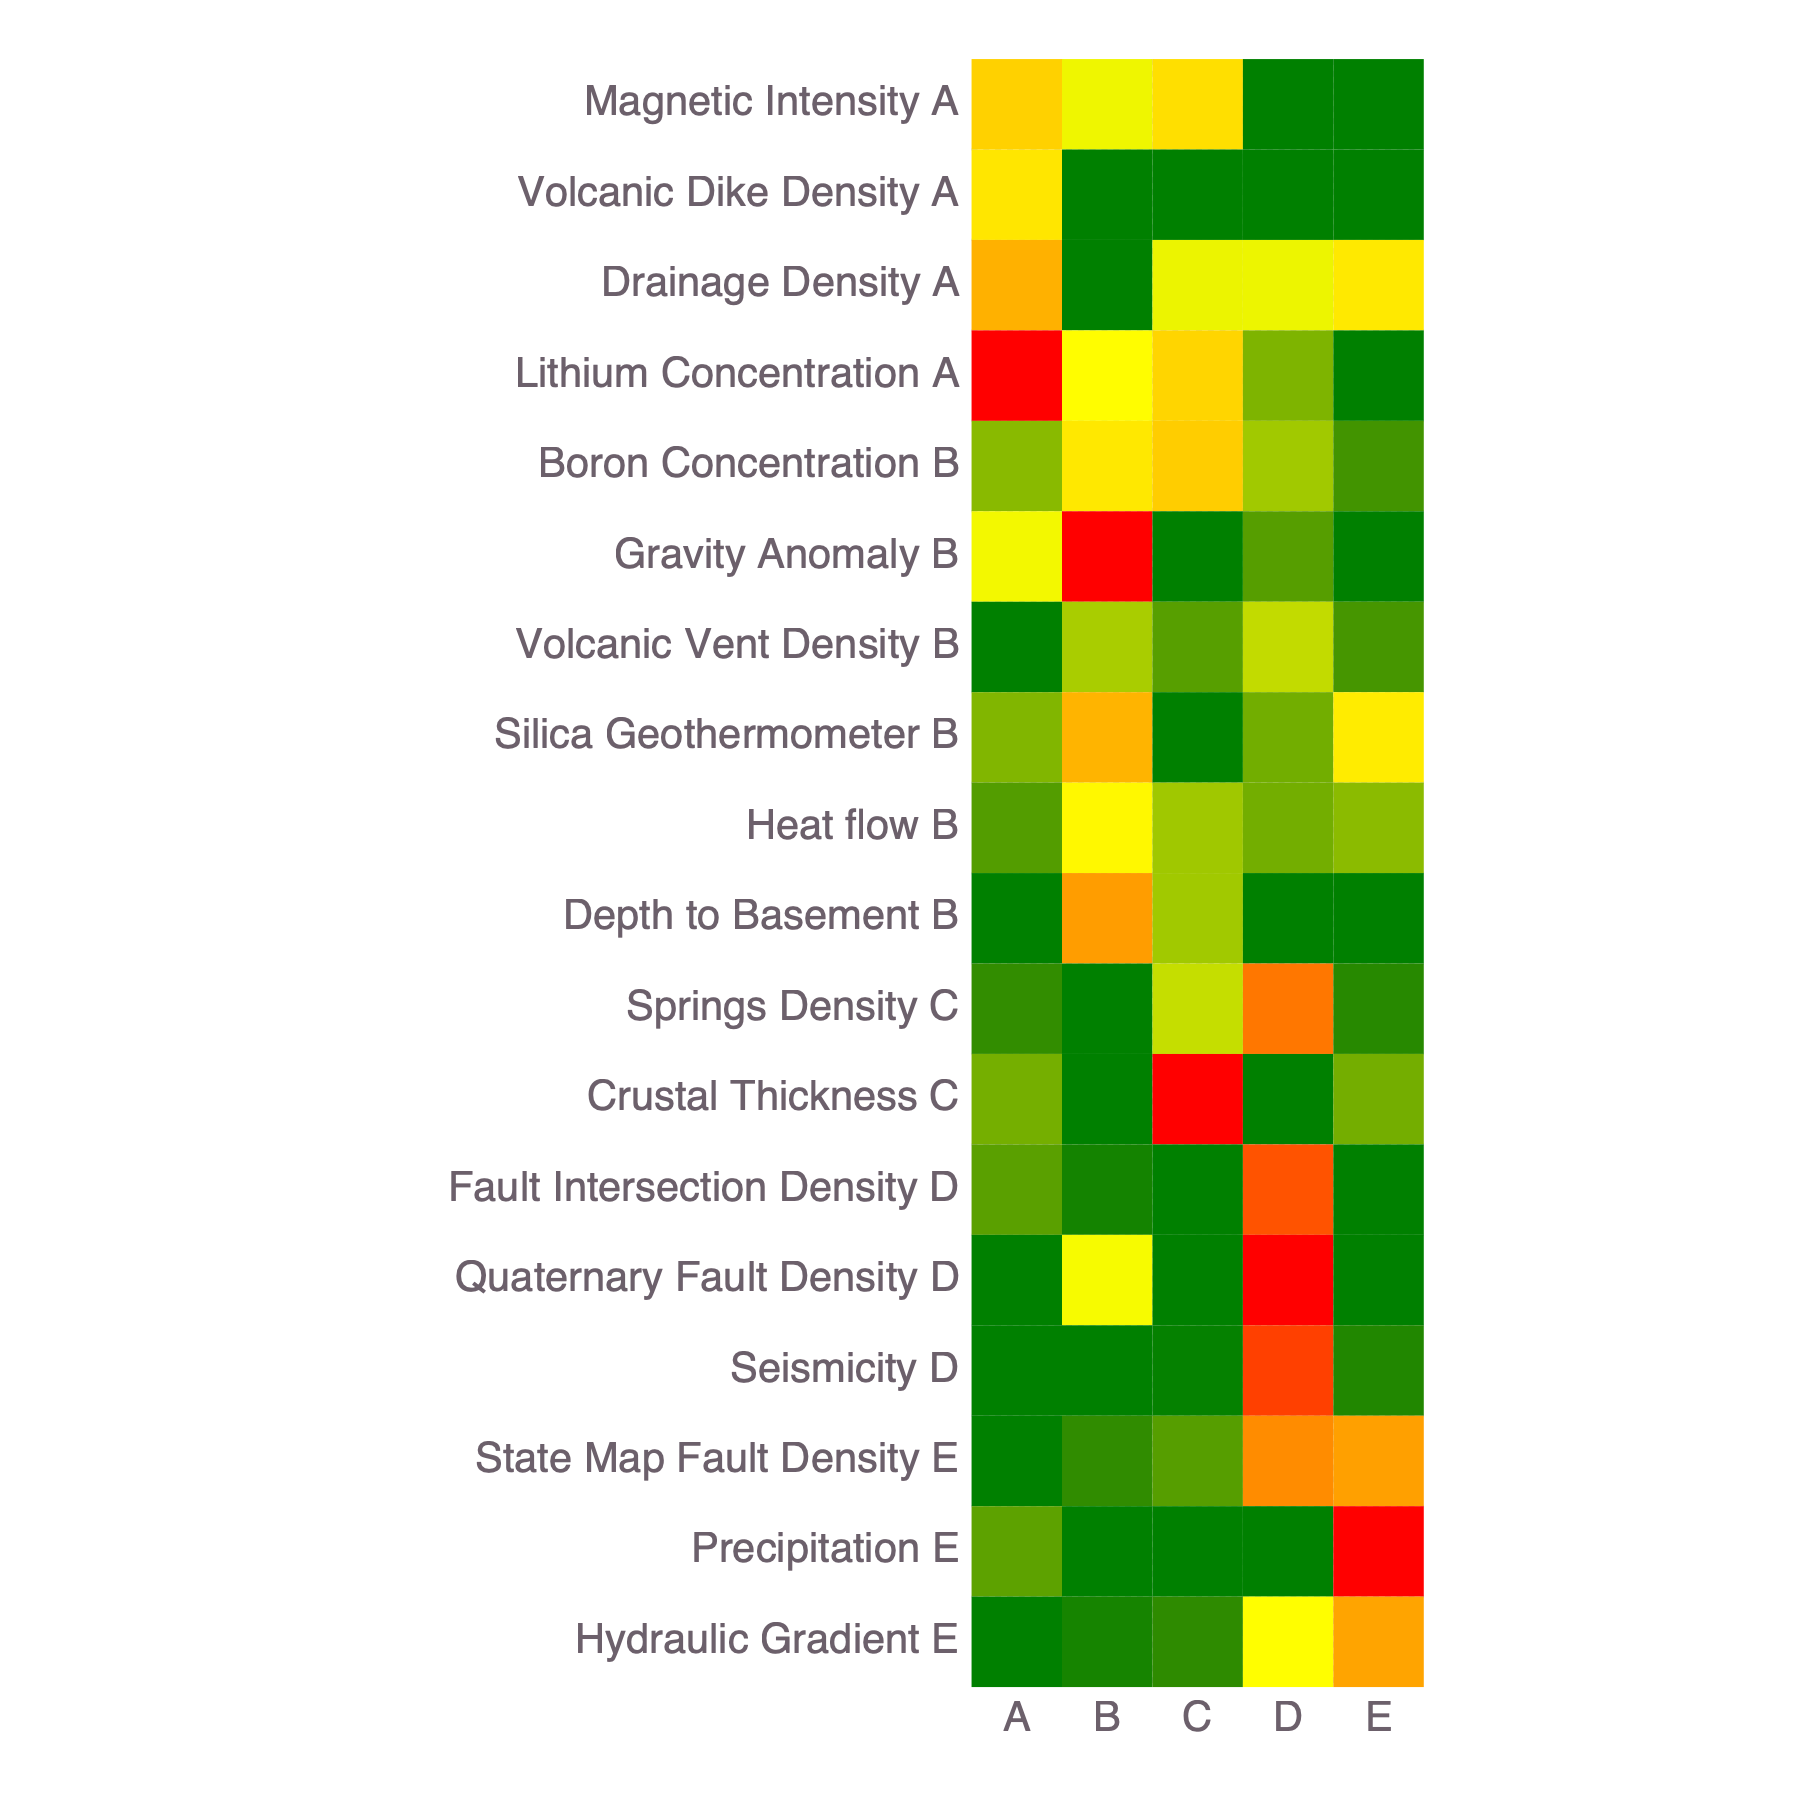
\includegraphics{../figures-case01/attributes-5-labeled-sorted.png}
\caption{attributes-3-labeled-sorted}
\end{figure}

The well locations are also clustered into \textbf{5} groups:

This grouping is based on analyses of the location matrix \texttt{H}:

\begin{figure}
\centering
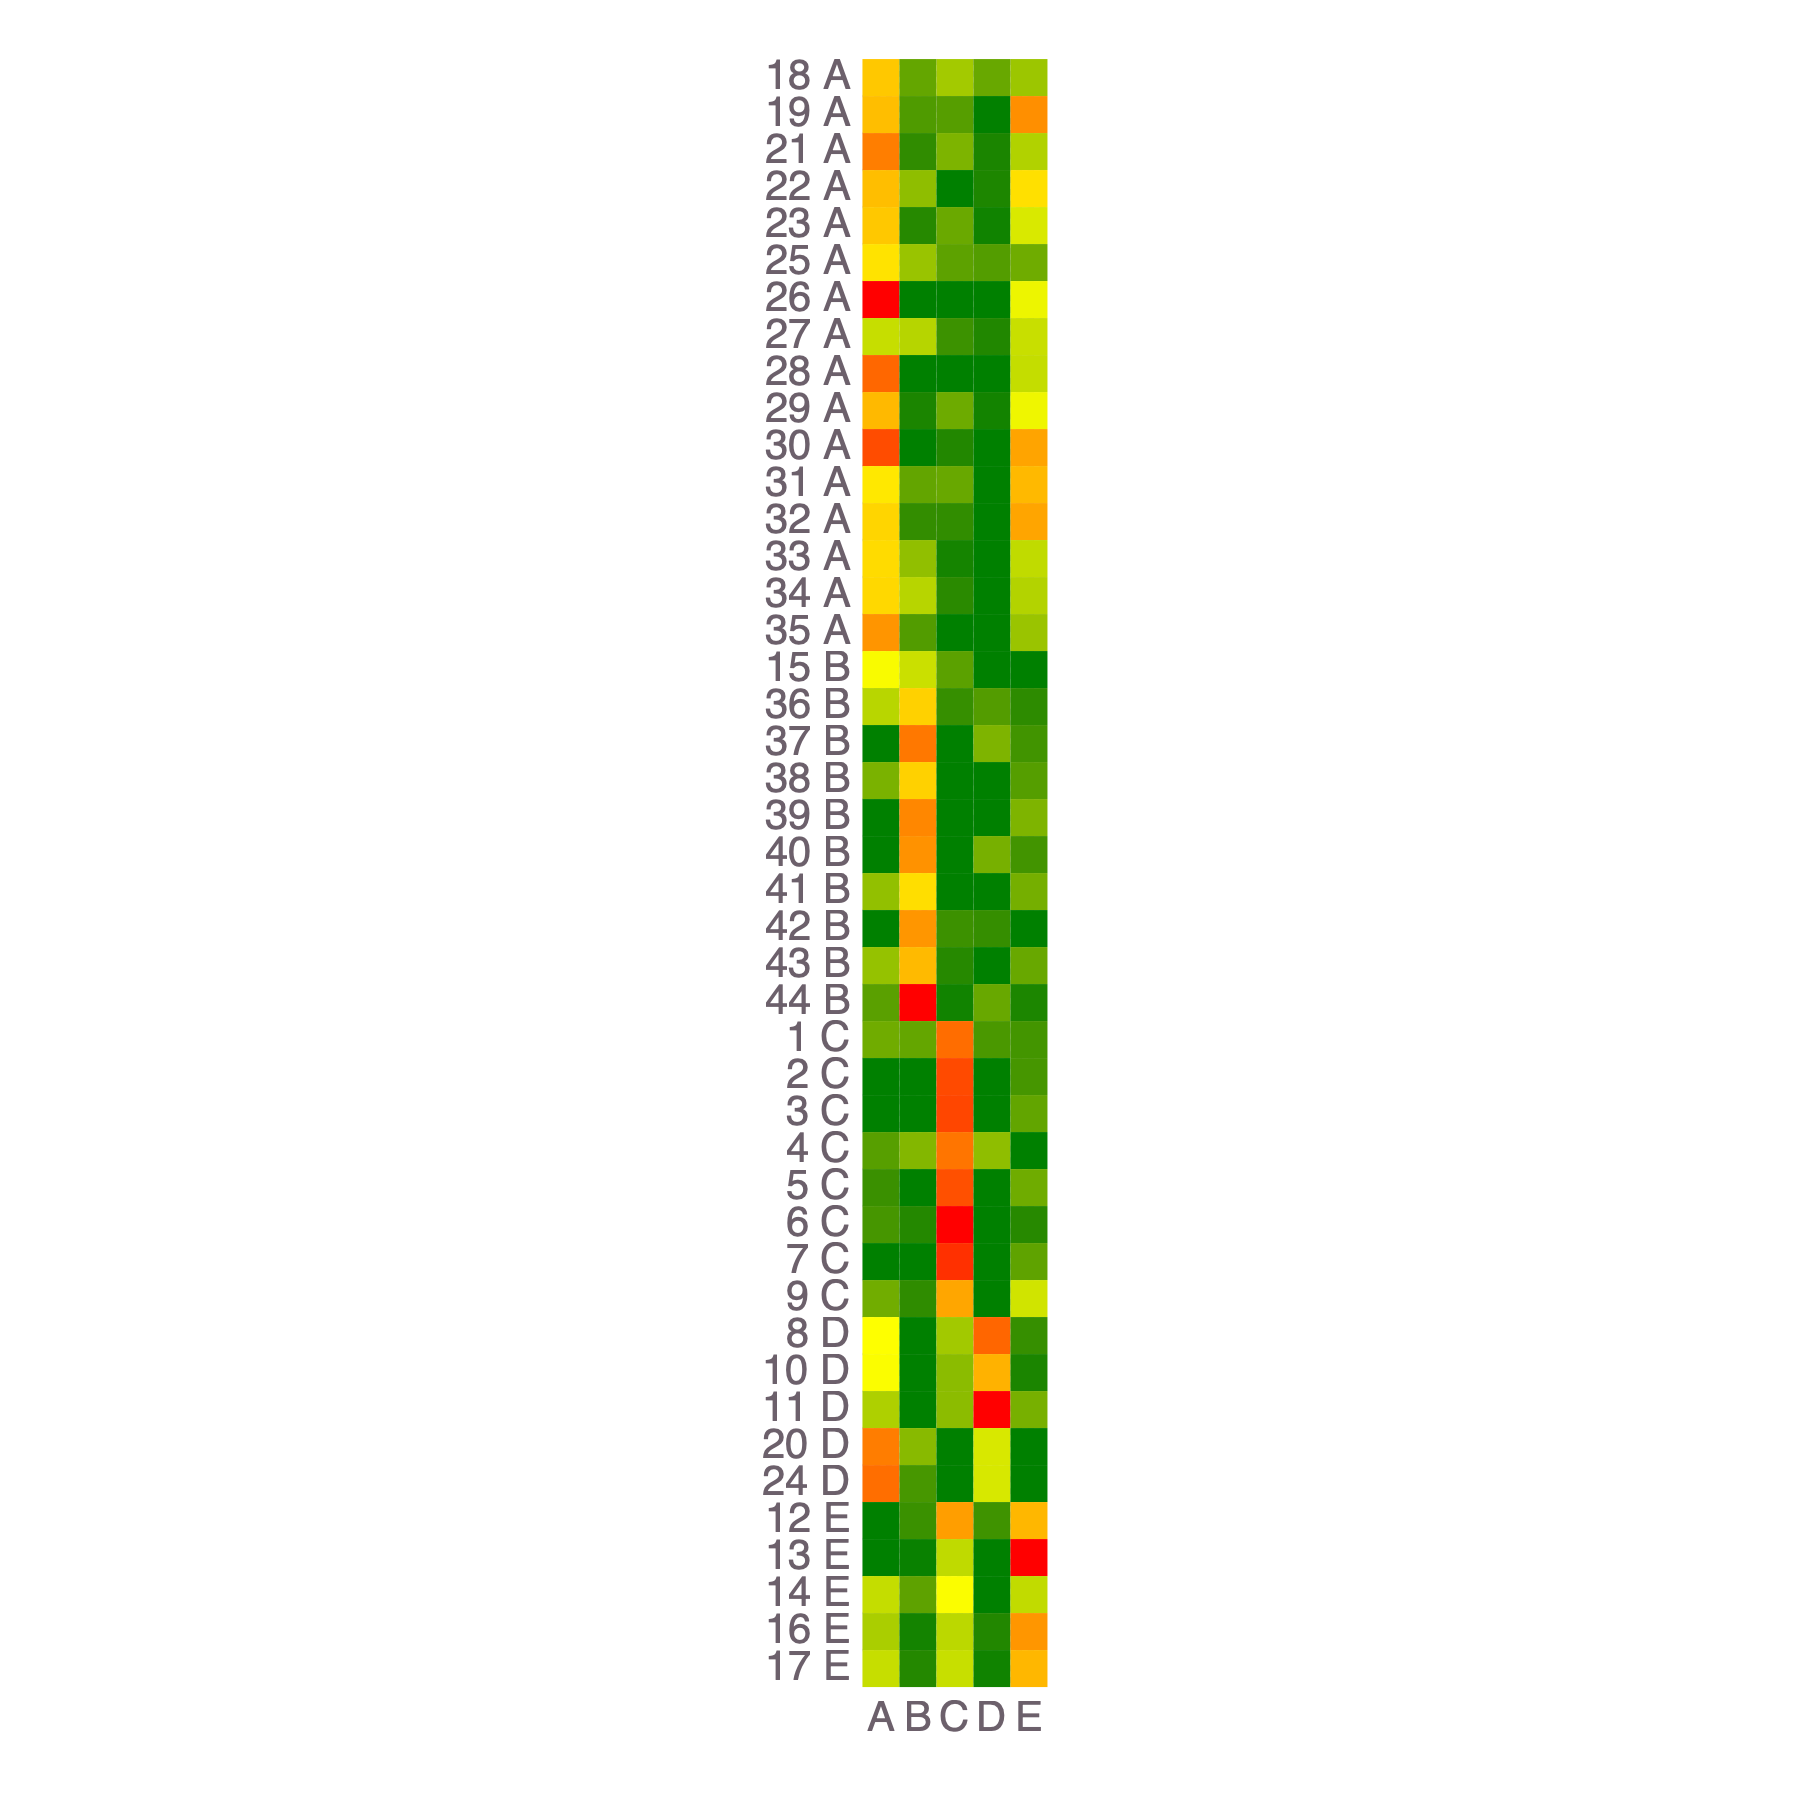
\includegraphics{../figures-case01/locations-5-labeled-sorted.png}
\caption{locations-4-labeled-sorted}
\end{figure}

The map \url{../figures-case01/locations-5-map.html} provides interacive
visualization of the extracted location groups (the html file can be
also openned with any browswer).

\begin{verbatim}
<iframe src="../figures-case01/locations-5-map.html" frameborder="0" height="400" width="50%"></iframe>
\end{verbatim}

    \hypertarget{comparison-of-the-ml-solutions-against-the-swnm-physiographic-provinces}{%
\paragraph{Comparison of the ML solutions against the SWNM physiographic
provinces}\label{comparison-of-the-ml-solutions-against-the-swnm-physiographic-provinces}}

Spatial association of the extracted signatures with the four
physiographic provinces in SWNM is summarized here:

\begin{figure}
\centering
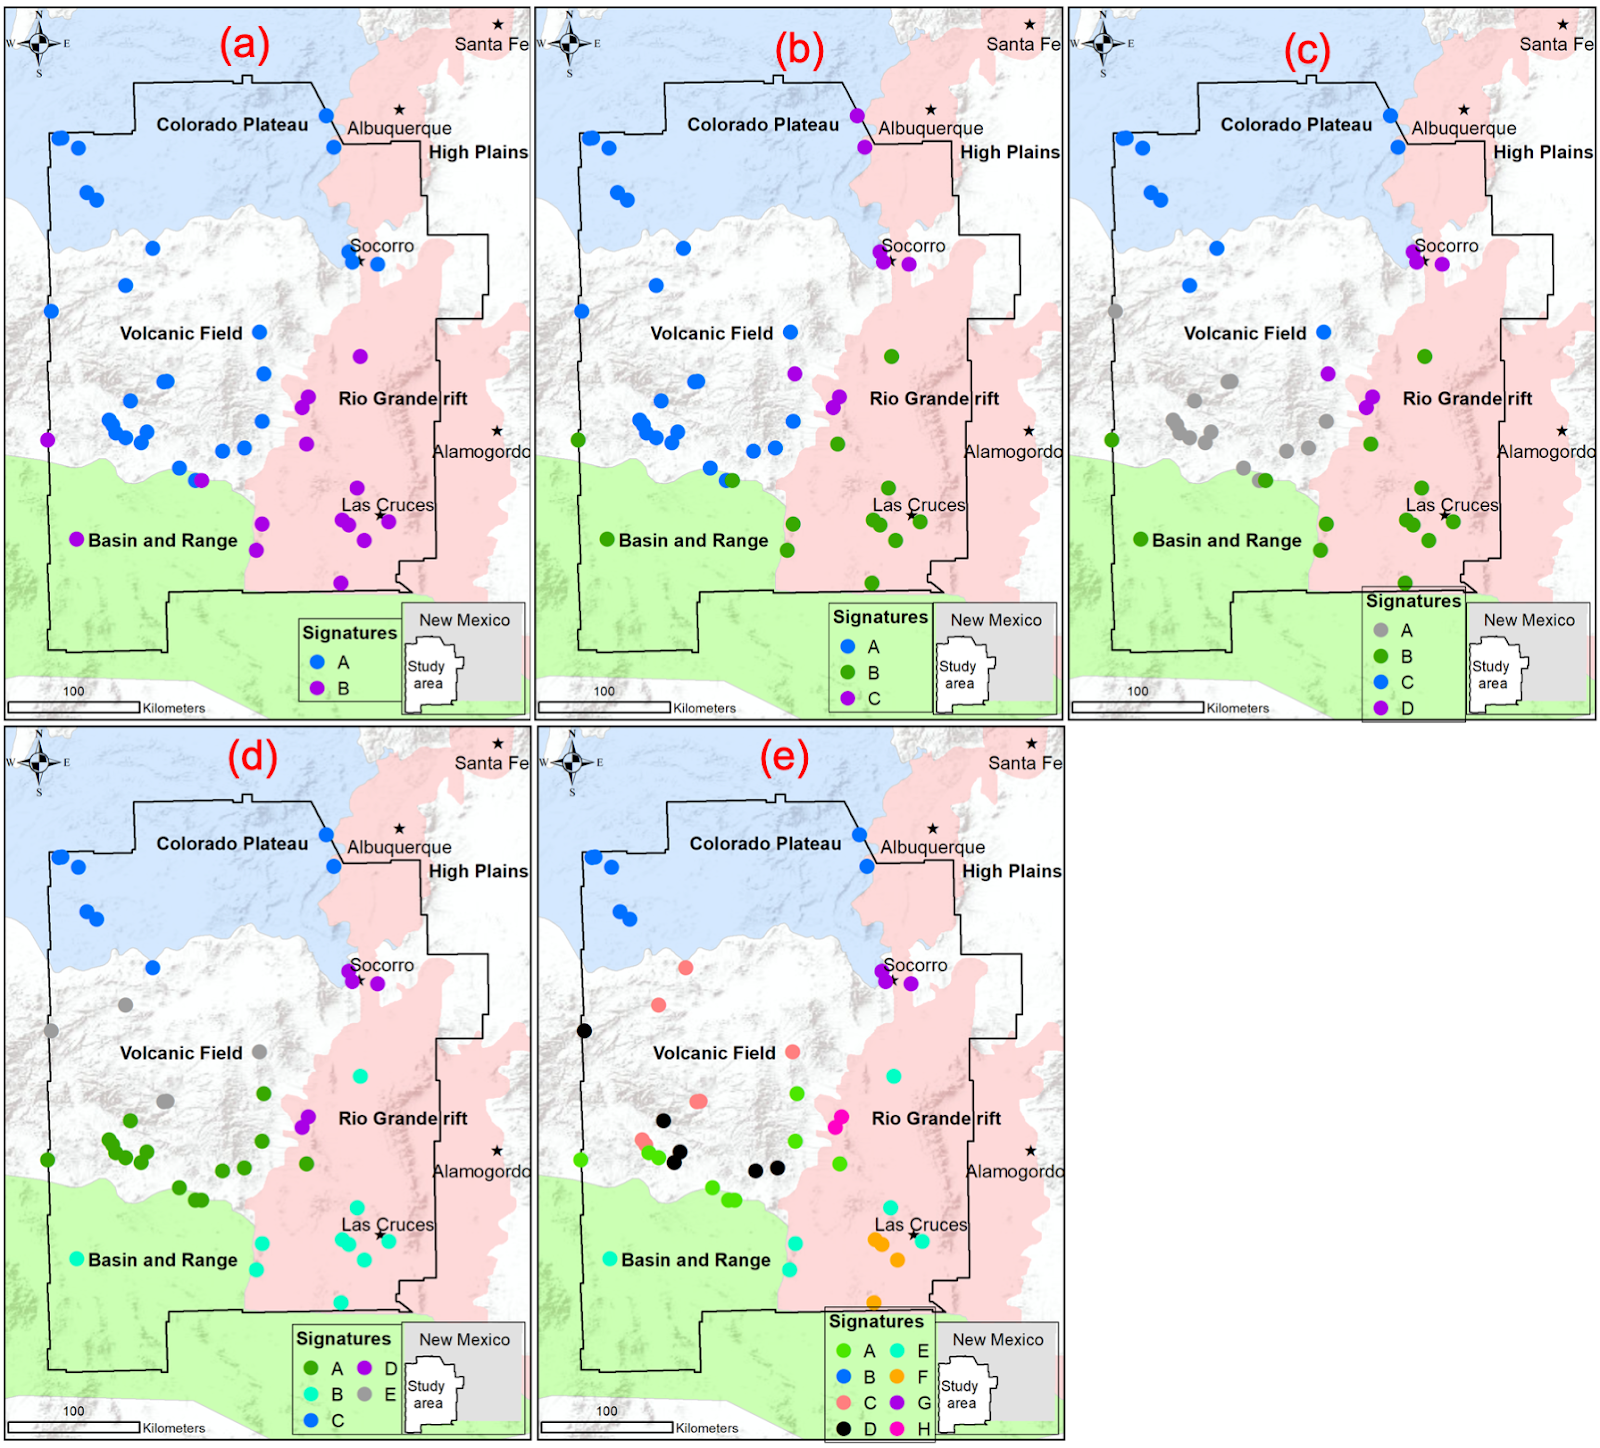
\includegraphics{../figures-case01/signatures.png}
\caption{signatures}
\end{figure}

Clearly, the ML algorithm was able to blindly indentify the
physiographic provinces associated with analyzed hydrogeothermal systems
without providing any information about their location (coordinates).


    % Add a bibliography block to the postdoc
    
    
    
\end{document}
